\chapter{Diverse logics encode notochord enhancers}

The notochord is a key structure during chordate development. We have previously identified several enhancers regulated by Zic and ETS that encode notochord activity within the marine chordate \textit{\textit{Ciona} robusta} (\textit{Ciona}). To better understand the role of Zic and ETS within notochord enhancers, we tested 90 genomic elements containing Zic and ETS sites for expression in developing \textit{Ciona} embryos using a whole-embryo, massively parallel reporter assay. We discovered that 39/90 of the elements were active in developing embryos; however only 10\% (9/90) were active within the notochord, indicating that more than just Zic and ETS sites are required for notochord expression. Further analysis revealed notochord enhancers were regulated by three groups of factors: (1) Zic and ETS, (2) Zic, ETS and Brachyury (Bra), and (3) Zic, ETS, Bra and FoxA. One of these notochord enhancers, regulated by Zic and ETS, is located upstream of \textit{laminin alpha}, a gene critical for notochord development in both \textit{Ciona} and vertebrates. Reversing the ETS sites in this enhancer greatly diminishes expression, indicating that enhancer grammar is critical for enhancer activity. Strikingly, we find clusters of Zic and ETS binding sites within the introns of mouse and human \textit{laminin alpha-1} with conserved enhancer grammar. Our analysis also identified two notochord enhancers regulated by Zic, ETS, FoxA and Bra binding sites: the Bra Shadow (BraS) enhancer located in close proximity to the gene \textit{Bra}, and an enhancer located near the gene \textit{Lrig}. By creating a library of 45 million enhancer variants with the sequence, affinity and position of the Zic, ETS, FoxA and Bra sites fixed while all other nucleotides are randomized, we discover that these sites are necessary and sufficient for notochord expression. Zic, ETS, FoxA and Bra binding sites occur within the \textit{Ciona} Bra434 enhancer and vertebrate notochord Bra enhancers, suggesting a conserved regulatory logic. Collectively, this study deepens our understanding of how enhancers encode notochord expression, illustrates the importance of enhancer grammar, and hints at the conservation of enhancer logic and grammar across chordates. 

%%%%%%%%%%%%%%%%%%%%%%%%%%%%%%%%%%%%%%%%%%%%%%%%%%%%%%%%%%%%%%%%%%%%%%%%%%%%%%%%
\section{Introduction}
%%%%%%%%%%%%%%%%%%%%%%%%%%%%%%%%%%%%%%%%%%%%%%%%%%%%%%%%%%%%%%%%%%%%%%%%%%%%%%%%

Enhancers are genomic elements that act as switches to ensure the precise patterns of gene expression required for development \cite{levine2010}. Enhancers regulate the timing, locations and levels of expression by binding of transcription factors (TFs) to sequences within the enhancer known as transcription factor binding sites (TFBSs) \cite{heinz2010,liu2012a,small1992,spitz2012,swanson2010a}. This binding, along with protein-protein interactions, leads to recruitment of transcriptional machinery and activation of gene expression. While we understand that TFBSs regulate enhancers and mediate tissue-specific expression, we have limited understanding of how the sequence of an enhancer encodes a particular expression pattern and what combinations of binding sites within enhancers are able to mediate enhancer activity. Given that the majority of variants associated with disease and phenotypic diversity lie within enhancers \cite{maurano2012a,tak2015a,visel2009}, it is critical that we understand how the underlying enhancer sequence encodes tissue-specific expression and what types of changes within an enhancer sequence can cause changes in expression, cellular identity and phenotypes. 

A set of grammatical rules that define how enhancer sequence encodes tissue-specific expression is an attractive idea first suggested almost 30 years ago \cite{arnone1997,barolo2016a,levo2014,thanos1995}. The hypothesis for grammatical rules is based on the fact that proteins and the enhancer DNA have physical properties. These physical constraints govern the interaction of proteins with DNA and could be read out within the DNA sequence at the level of TFBSs. Enhancer grammar is composed of constraints on the number, type, and affinity of TFBSs within an enhancer and the relative syntax of these sites (orders, orientations, and spacings) \cite{jindal2021}.

We previously identified grammatical rules governing notochord enhancers regulated by Zic and ETS TFBSs \cite{farley2016}. We found that there was an interplay between affinity and organization of TFBSs, such that organization could compensate for poor affinity and vice versa. Using these rules, we identified two novel notochord enhancers, Mnx and Bra Shadow (BraS). These enhancers use low-affinity ETS sites in combination with Zic sites to encode notochord expression \cite{farley2016}. Here, we focus on obtaining a deeper understanding of how enhancers regulated by Zic and ETS encode notochord expression. 

Zic and ETS are co-expressed in the developing notochord of the marine chordate \textit{Ciona} (Figure ~\ref{fig:1 zic ets expression}) and in vertebrates \cite{dykes2018,matsumoto2007a}. The notochord is a key feature of chordates and acts as a signaling center to pattern the neighboring neural tube, paraxial mesoderm, and gut \cite{herrmann1994,stemple2005}. Specification of the notochord by Brachyury (Bra), also known as T, is highly conserved across chordates \cite{chesley1935,chiba2009,wilkinson1990,yasuo1993}. Other conserved TFs important for activation of notochord gene expression include Zic, ETS, a TF downstream of FGF signaling, and FoxA \cite{ang1994,dal-pra2011,dykes2018,elms2004,imai2002,imai2002a,jose-edwards2015a,katikala2013,kumano2006,matsumoto2007a,matsumoto2007a,miya2003,passamaneck2009a,schulte-merker1995,warr2008,weinstein1994,yagi2004,yasuo2007}.

Our study focuses on the marine chordate, \textit{\textit{Ciona} intestinalis type A},  also known as \textit{\textit{Ciona} robusta} (\textit{Ciona}), a member of the urochordates, the sister group to vertebrates \cite{delsuc2006}(Delsuc et al., 2006). Fertilized \textit{Ciona} eggs can be electroporated with many enhancers in a single experiment which allows for testing of many enhancers in whole, developing embryos \cite{davidson2006,farley2015a}. Furthermore, these embryos are transparent and have defined cell lineages, making it easy to image and determine the location of enhancer activity. These advantages, along with the fast development of \textit{Ciona} and the similarity of notochord development programs between \textit{Ciona} and vertebrates \cite{davidson2006,digregorio2020}, make it an ideal organism to study the rules governing notochord enhancers during development. 

Within the \textit{Ciona} genome, we found 1,092 elements containing one Zic site and at least two ETS sites within 30 bp upstream or downstream of the Zic site. We tested 90 of these for expression in developing \textit{Ciona} embryos. Only 10\% of these regions drive notochord expression. These notochord enhancers fall into three categories: enhancers containing Zic and ETS sites, ones with Zic, ETS and Bra sites, and ones with Zic, ETS, FoxA and Bra sites. Within enhancers containing Zic and ETS sites, the organization of sites is important for activity, indicating that grammatical constraints on Zic and ETS encode enhancer activity. We find that one of the Zic and ETS enhancers is near an important notochord gene, \textit{laminin alpha} \cite{veeman2008}. The orientation of binding sites within this \textit{laminin alpha} enhancer is critical for enhancer activity demonstrating the role of enhancer grammar.  We find similar clusters of Zic and ETS sites within the introns of \textit{laminin alpha-1} in both mouse and human. Strikingly, we find the same 12 bp spacing between the Zic and ETS conserved across all three species. Additionally, this study identifies two enhancers using a combination of Zic, ETS, FoxA, and Bra to encode notochord expression. One of these is the BraS enhancer. By creating a library of 45 million enhancer variants with the sequence, affinity and position of the Zic, ETS, FoxA and Bra sites fixed while all other nucleotides are randomized, we discover that these sites are necessary and sufficient for notochord expression. Other known Bra enhancers within \textit{Ciona} \cite{corbo1997} and vertebrates \cite{schifferl2021} also harbor this combination of TFs, suggesting that Zic, ETS, FoxA, and Bra is a common feature of Bra regulation in chordates. Collectively, our study finds that grammar is a key component of functional enhancers with signatures of this enhancer logic and grammar seen across chordates. 

\begin{figure}[h]
    \centering
    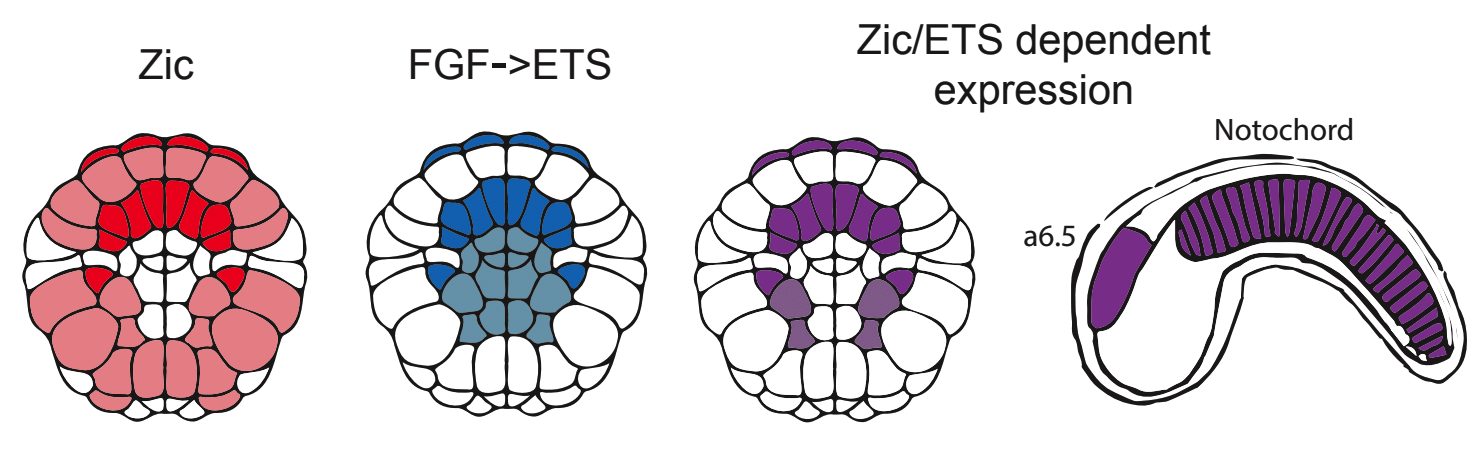
\includegraphics[scale=0.25]{2_figures/Fig1_ZicEts-Expression.png}
    \caption[Zic and ETS expression in the 110-cell stage embryo]{\textbf{Zic and ETS expression in the 110-cell stage embryo.} Co-expression of Zic and ETS is shown in purple and occurs in the notochord, a6.5 lineage, which gives rise to the anterior sensory vesicle and palps, and four mesenchyme cells shown in light purple. A schematic of the tailbud embryo shows the notochord and a6.5 cell types later in development. Dark coloring represents a6.5 and notochord lineages, and light coloring represents other tissues with expression of Zic and/or ETS.}
    \label{fig:1 zic ets expression}
\end{figure}

%%%%%%%%%%%%%%%%%%%%%%%%%%%%%%%%%%%%%%%%%%%%%%%%%%%%%%%%%%%%%%%%%%%%%%%%%%%%%%%%
\section{Results}
%%%%%%%%%%%%%%%%%%%%%%%%%%%%%%%%%%%%%%%%%%%%%%%%%%%%%%%%%%%%%%%%%%%%%%%%%%%%%%%%

\subsection{Searching for clusters of Zic and ETS sites within the \textit{Ciona} genome}

To better understand how Zic and ETS sites within enhancers encode notochord expression, we searched the \textit{Ciona} genome (KH2012) for clusters of Zic and ETS sites. To do this, we first identified Zic motifs in the genome. We defined Zic motifs using EMSA and enhancer mutagenesis data from previous studies (see methods for motifs) \cite{matsumoto2007a,takahashi1999,yagi2004}. Using the Zic site as an anchor, we searched the 30 bp upstream and downstream of  the Zic site for ETS sites, using the core motif \verb|GGAW| (\verb|GGAA| and \verb|GGAT|) to consider all ETS sites regardless of affinity \cite{lamber2008,wei2010}, as we have previously found that low-affinity ETS sites are required to encode notochord-specific expression \cite{farley2016}. This search identified 1,092 genomic regions approximately 68 bp in length. We define these regions as ZEE elements. 

\subsection{Testing ZEE genomic elements for enhancer activity in developing \textit{Ciona} embryos}

We selected 90 ZEE elements (Figure ~\ref{fig:supplement zee elements screened}1 and Table S1) and synthesized these upstream of a minimal promoter (bpFog) \cite{rothbacher2007,stolfi2015} and a transcribable barcode to conduct an enhancer screen (experiment outlined in Figure ~\ref{fig:2 enhancer screen schematic}A). Each enhancer was associated with, on average, six unique barcodes. Each different barcode is a distinct measurement of enhancer activity. We electroporated this library into fertilized \textit{Ciona} eggs. We collected embryos at the late gastrula stage (5.5 hours post fertilization, hpf) when notochord cells are developing \cite{jiang2007} and both Zic and ETS are expressed \cite{imai2004,winkley2021}. At this timepoint, we isolated mRNA and DNA. To determine that all the enhancer plasmids got into the embryos, we isolated the plasmids from the embryos and sequenced the DNA barcodes. We detected barcodes associated with all 90 ZEE elements from the isolated plasmids, indicating that all elements were tested for activity within the developing \textit{Ciona} embryos. 

We next wanted to see how many of the 90 ZEE elements act as enhancers to drive transcription. Active enhancers will transcribe the GFP and the barcode into mRNA. To find the functional enhancers, we isolated the mRNA barcodes from our electroporated embryos and sequenced them. We analyzed the sequencing data and measured the reads per million (RPM) for each barcode. To calculate an average RNA RPM for a given enhancer, we averaged the RPM for each RNA barcode associated with an enhancer. To normalize the enhancer activity to the differences in the amount of plasmid and therefore number of copies of the enhancer electroporated into embryos, we took the $log_2$ of the average enhancer RNA RPM divided by the DNA RPM for the same enhancer to create an enhancer activity score. Enhancer activity scores below zero are non-functional, while elements with scores above zero are considered functional enhancers. The highest activity score is around four. The experiment was repeated in biological triplicate and there was a high correlation between all three biological replicates (Figure ~\ref{fig:supplement notochord data qc}).

\begin{figure}[p]
    \centering
    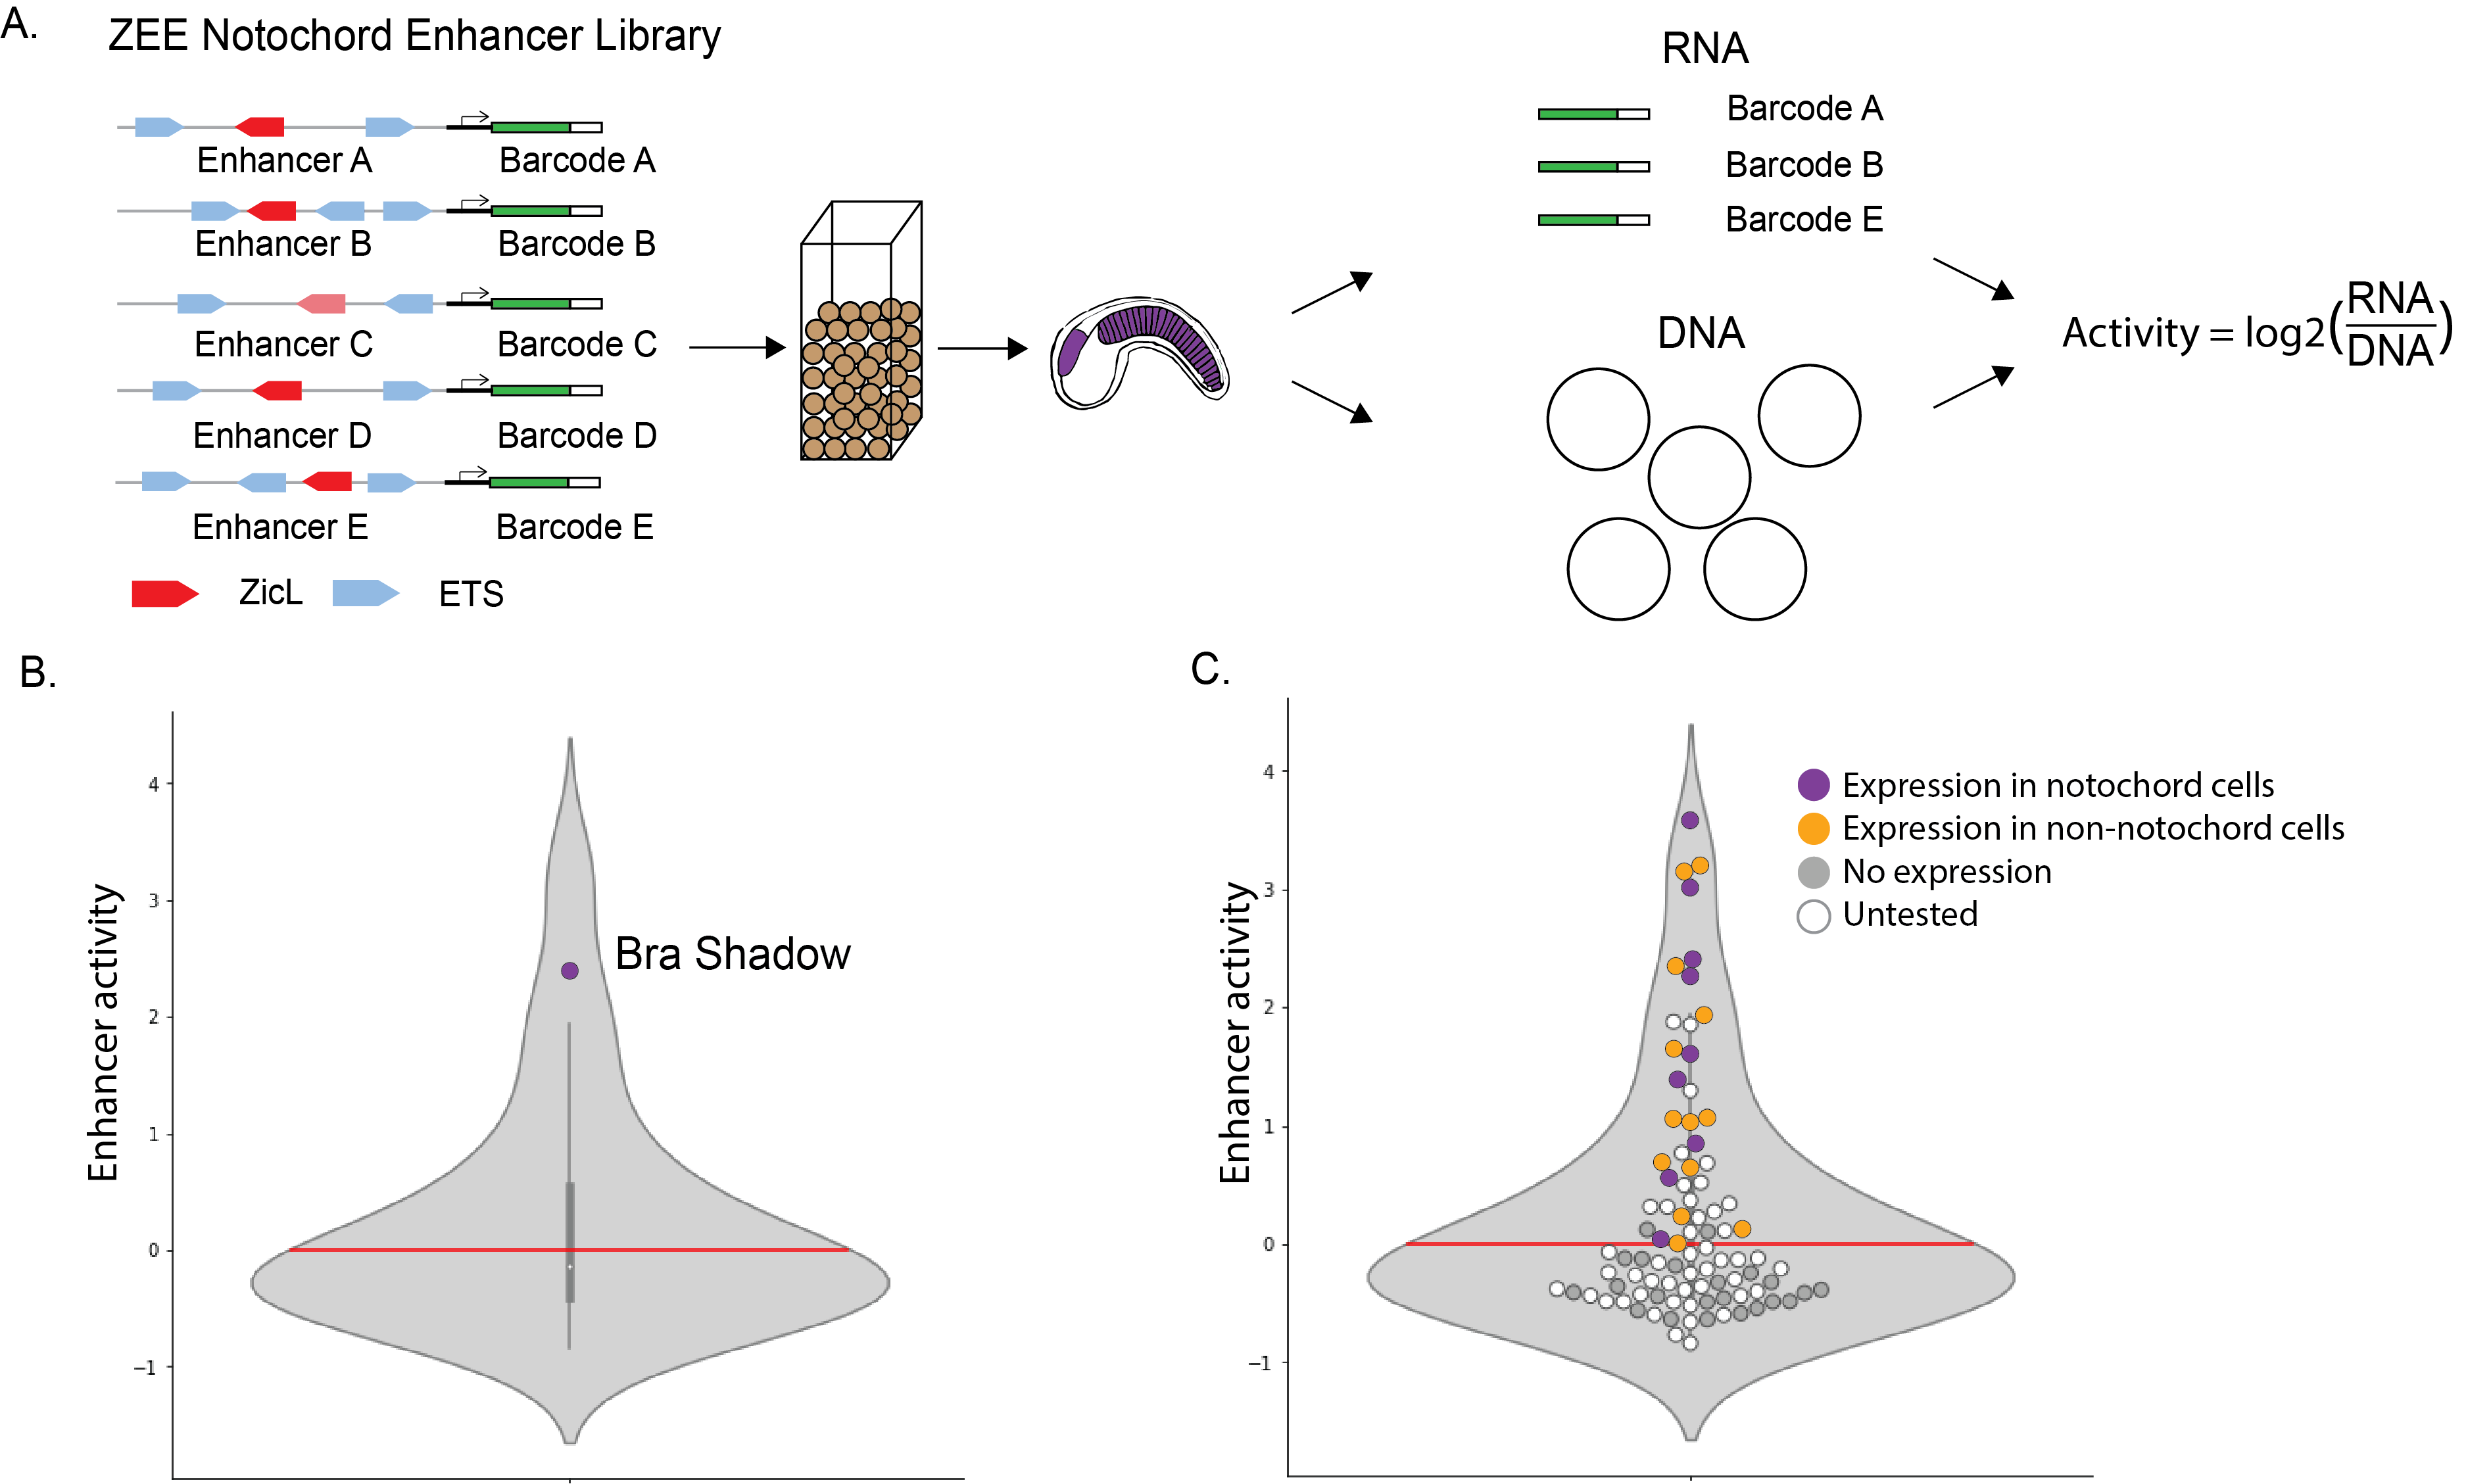
\includegraphics[scale=.5]{2_figures/Fig2_Enhancer-Screen_Expression-Distribution.png}
    \caption[Screening Zic and ETS genomic elements in \textit{Ciona}]{\textbf{Screening Zic and ETS genomic elements in \textit{Ciona}.} \textbf{A.} Schematic of enhancer screen. 90 ZEE genomic regions, each associated with on average six unique barcodes were electroporated into fertilized \textit{Ciona} eggs. mRNA and plasmid DNA were extracted from 5.5 hpf embryos (tailbud embryo shown to highlight tissues with predicted expression). The mRNA and DNA barcodes were sequenced, and a normalized enhancer activity score was calculated for each enhancer by taking the $log_2$ of the mRNA activity for a given enhancer divided by the number of copies of the plasmid. \textbf{B.} Violin plot showing the distribution of enhancer activity. The Bra Shadow enhancer served as a positive control and is labeled. The red line indicates the cut-off for non-functional elements at zero. \textbf{C.} Same plot as (B), but with all 90 ZEE elements plotted as dots. Dots are colored by the results of an orthogonal screen, where we measured the GFP expression in at least 150 embryos to determine the location of expression (50 embryos per repeat). Enhancers driving notochord expression are shown in purple, enhancers with expression but no notochord expression are shown in orange. ZEE elements that do not drive expression are grey and untested enhancers are shown in white.}
    \label{fig:2 enhancer screen schematic}
\end{figure}

\subsection{Many genomic ZEE elements are not enhancers}

As an internal, positive control in our enhancer screen, we included the Bra Shadow (BraS) enhancer. This enhancer drives expression in the notochord and weak expression in the a6.5 lineage, both locations that express Zic and ETS \cite{farley2016}. The BraS enhancer activity score is 2.4 (Figure ~\ref{fig:2 enhancer screen schematic}B), indicating that our library screen is detecting functional enhancers. Thirty-nine of the ZEE elements act as enhancers in our screen, while fifty-one of the ZEE elements drove no expression. This suggests that genomic elements containing a single Zic site and at least two ETS sites are not sufficient to drive expression in the notochord. To further validate our sequencing data and to determine the tissue-specific location of the functional enhancers, we selected 20 non-functional elements and 24 functional enhancers from our screen to test by an orthogonal approach. Each of these ZEE elements were cloned upstream of a minimal bpFog promoter and GFP. We electroporated each enhancer into fertilized eggs and analyzed the GFP expression of these ZEE elements under the microscope at 8 hpf in at least 150 embryos across three biological replicates. Collectively, we analyzed expression of these elements in over 6,600 embryos with this orthogonal approach. 

All 20 ZEE elements defined as non-functional in our library drove no GFP expression, validating our enhancer activity score cut off that we defined for non-functional enhancers (Figure ~\ref{fig:2 enhancer screen schematic}C). In the 24 enhancers detected as functional within the enhancer screen, 92\% of these enhancers (22/24) showed GFP expression within the embryos when tested individually (Table S2). Nine ZEE elements drove expression in the notochord (Figure ~\ref{fig:supplement all notochord enhancers}3 and Table S3). Four of these enhancers are active almost exclusively in the notochord (ZEE10, 13, 20, 27). The remaining five are active in the notochord with additional expression in the endoderm and/or nerve cord (b6.5 lineage). Twelve of the ZEE enhancers drove varying levels of expression in the a6.5 lineage, which gives rise to the neural cell types called the anterior sensory vesicle and the palps, but only one drove expression exclusively in this cell type (ZEE22). Thirteen ZEE elements drove expression in one or more for the following cell types: the nerve cord (b6.5 lineage), mesenchyme, and endoderm. The expression patterns seen for these active enhancers are consistent with the expression patterns of Zic and ETS which are expressed in the muscle, endoderm, ectoderm, mesenchyme, notochord, a6.5 neural lineage and b6.5 neural cell types \cite{hudson2007,hudson2016,imai2006,picco2007,wagner2012} (Note, S1 discusses the expression patterns of the ZEE elements with notochord expression in more detail). The only cells to co-express both Zic and ETS are the notochord, a6.5, and a small number of mesenchyme cells (Figure ~\ref{fig:1 zic ets expression}). Therefore, enhancers under combinatorial control of Zic and ETS are likely to be active in the notochord and the a6.5 neural lineage \cite{ikeda2016,matsumoto2007a,wagner2012}. Collectively these results indicate that our enhancer screen accurately detects functional enhancers, and our tissue-specific analysis provides detailed expression patterns for these enhancers. 

\subsection{Elucidating the logic of the enhancers driving notochord expression}

Having seen that so few enhancers drive expression in the notochord, we were interested to better understand why these nine functional enhancers were active in the notochord. It is possible that they are functional due to the grammar of the Zic and ETS sites or because other TFBSs are required for notochord expression. To investigate these two hypotheses, we looked at the nine notochord enhancers in more detail. FoxA and Bra are two other TFs important for activation of notochord enhancers in chordates \cite{ang1994,casey1998,dal-pra2011,jose-edwards2015a,katikala2013,passamaneck2009a,wilkinson1990}. We therefore searched all 90 ZEE elements for FoxA and Bra sites. We used EMSA and crystal structure data to define \verb|TRTTTAY| as the FoxA motif \cite{katikala2013,li2017,passamaneck2009a} and \verb|TNNCAC| as the Bra motif \cite{casey1998,conlon2001,digregorio1999,dunn2009,muller1997}. 

\begin{figure}[h]
    \centering
    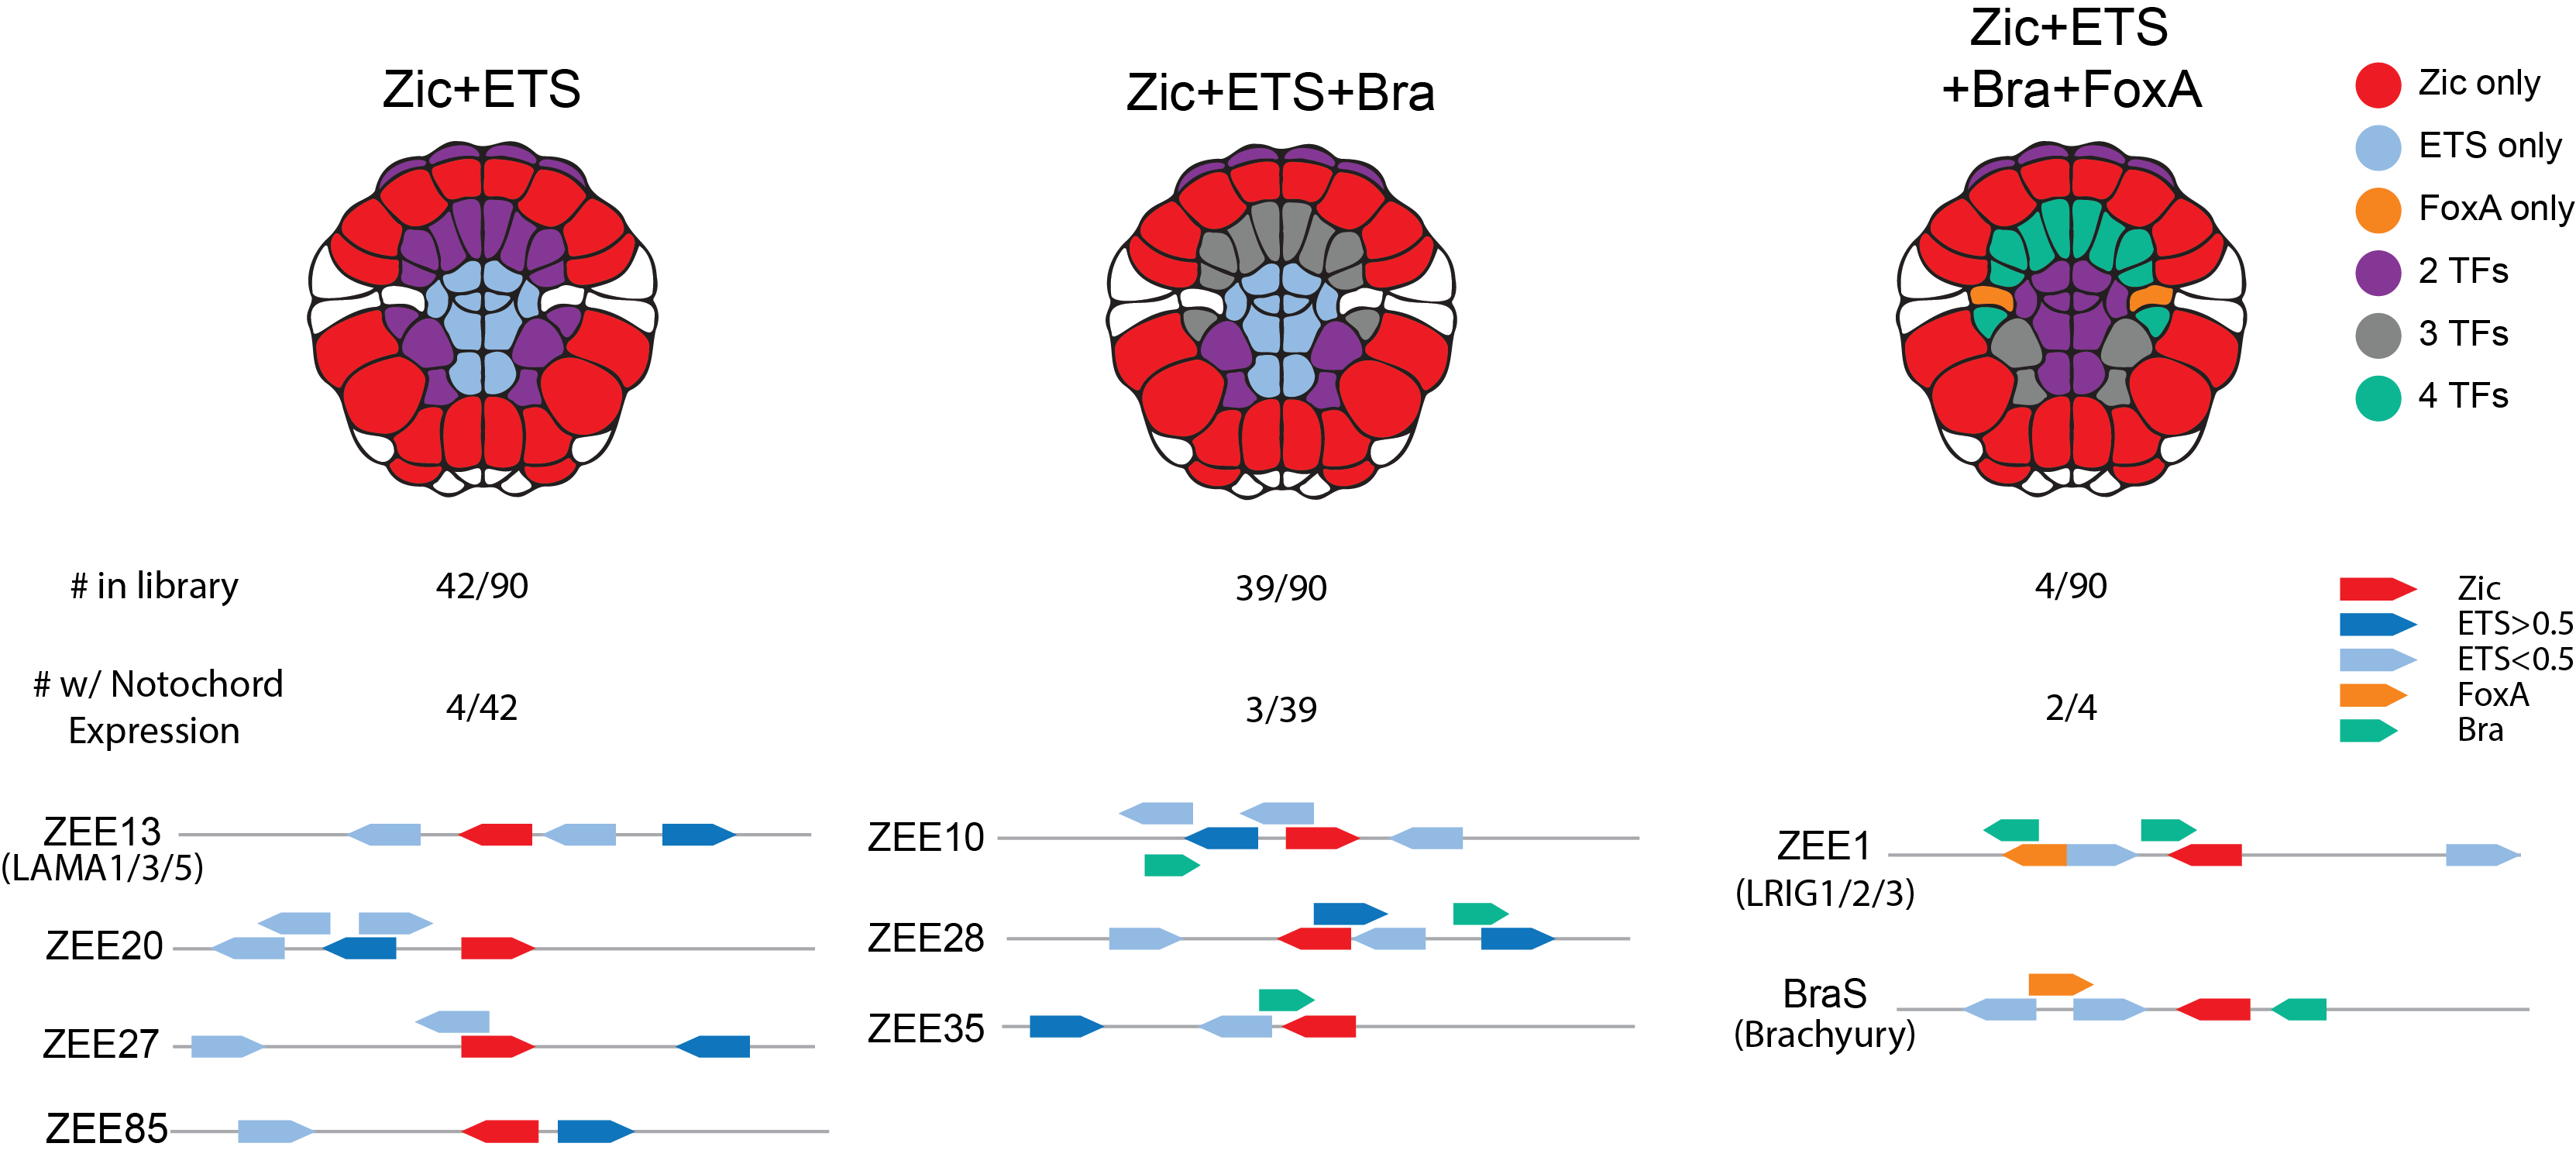
\includegraphics[scale=.55]{2_figures/Fig3_Notochord-Grammar-Groups.png}
    \caption[Combinations of transcription factors in ZEE enhancers that drive notochord expression]{\textbf{Combinations of transcription factors in ZEE enhancers that drive notochord expression.} Notochord-expressing ZEE elements were grouped by the combination of transcription factor binding sites present in each element. For each combination, an embryo schematic shows the overlapping region of expression for that given combination. Below the embryo schematic, the number of ZEE elements, the number of ZEE elements with notochord expression and schematics of the ZEE elements with notochord expression within each group. Zic (red), ETS (blue), FoxA (orange), and Bra (green) sites are annotated. Dark blue ETS sites have an affinity of greater than 0.5, light blue sites have an affinity of less than 0.5.}
    \label{fig:3 notochord enhancer groups}
\end{figure}

\subsection{The nine elements that drive notochord expression contain three different combinations of transcription factors}

Of the 90 genomic regions we tested, 42 had only Zic and ETS sites, 39 had Zic, ETS and Bra sites, 4 had Zic, ETS, FoxA, and Bra sites and 5 had Zic, ETS and FoxA sites. Ten percent of the enhancers containing only Zic and ETS sites drive notochord expression (4/42). Eight percent (3/39) of the enhancers containing Zic, ETS, and Bra drive notochord expression. None of the enhancers (0/5) containing Zic, ETS, and FoxA drive notochord expression, while fifty percent (2/4) of the enhancers containing Zic, ETS, FoxA and Bra are active in the notochord (Figure ~\ref{fig:3 notochord enhancer groups} and Figure ~\ref{fig:supplement annotated zee elements}). Thus, there are three groups of notochord enhancers that contain: (1) Zic and ETS sites alone, (2) Zic, ETS and Bra sites, or (3) Zic, ETS, FoxA, and Bra sites. Having found that only a few of the elements containing Zic and ETS sites alone were functional, we wanted to understand if the organization or grammar of sites within these enhancers was important.

\begin{figure}[p]
    \centering
    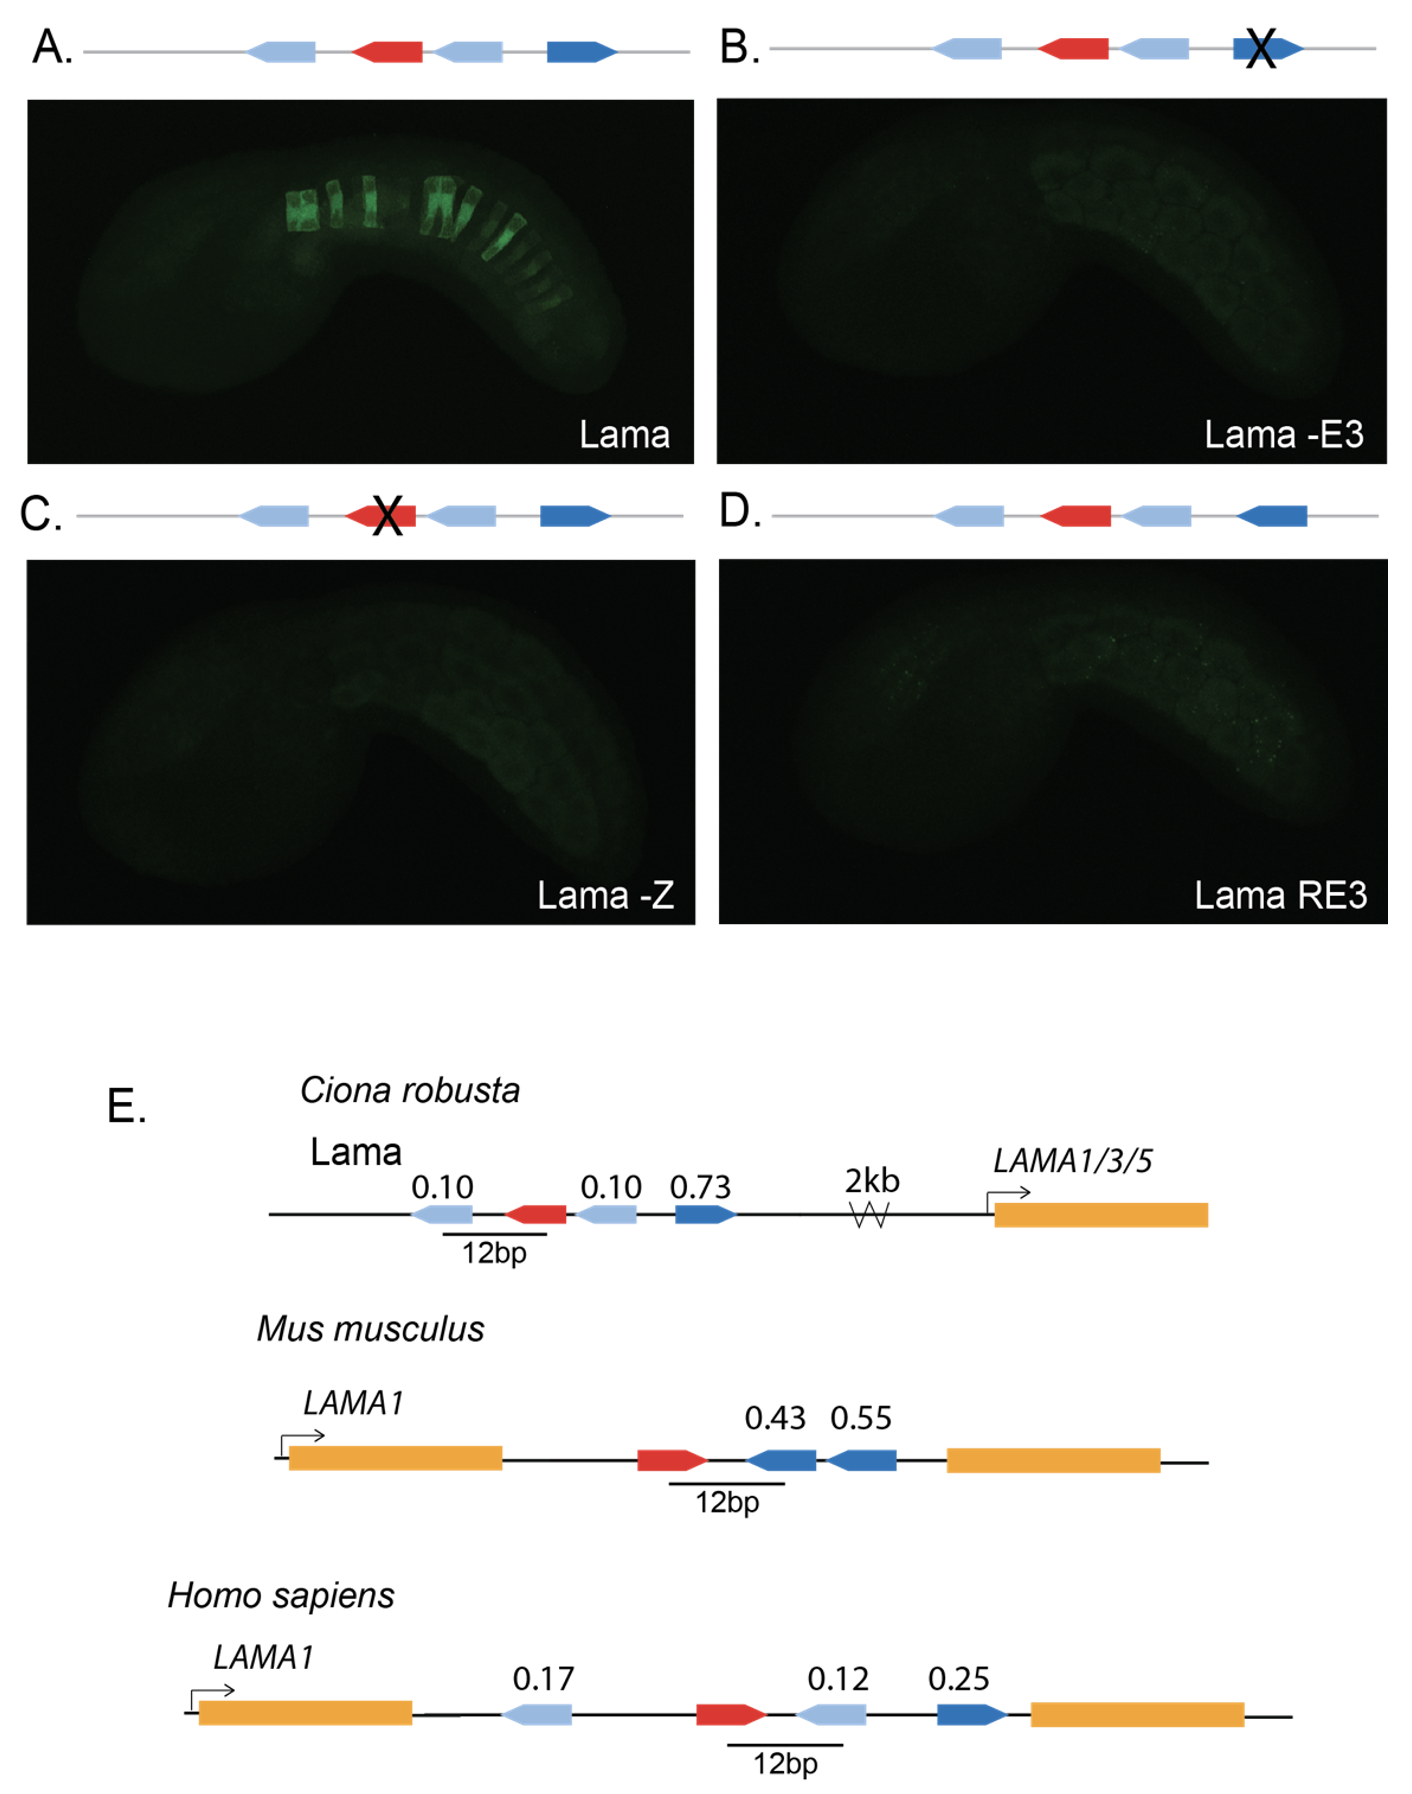
\includegraphics[scale=.52]{2_figures/Fig4_Laminin-alpha-Enhancer.png}
    \caption[Zic and ETS grammar encodes a notochord \textit{laminin alpha} enhancer]{\textbf{Zic and ETS grammar encodes a notochord \textit{laminin alpha} enhancer.} \textbf{A.} Embryo electroporated with the Lama enhancer (ZEE13); GFP expression can be seen in the notochord. \textbf{B.} Embryo electroporated with Lama -E3, where ETS3 was mutated to be non-functional; no GFP expression detected. \textbf{C.} Embryo electroporated with Lama -Z, where the Zic was mutated to be non-functional; no GFP expression detected. \textbf{D.} Embryo electroporated with Lama RE3, where the sequence of ETS3 was reversed; no GFP expression detected. Comparable results were seen when ETS1 was reversed. \textbf{E.} Schematics of Zic and ETS clusters near \textit{laminin alpha}  in the genome of \textit{Ciona}, mouse, and human. All three \textit{laminin alpha}  clusters have a spacing of 12 bp between an ETS and Zic site and all contain non-consensus ETS sites. ETS site affinity scores are noted above each site. Dark blue ETS sites have an affinity of greater than 0.5, light blue sites have an affinity of less than 0.5.}
    \label{fig:4 laminin alpha enhancer}
\end{figure}

\subsection{Zic and ETS enhancer grammar encodes notochord \textit{laminin alpha}  expression}

Four enhancers containing Zic and ETS sites only (ZEE13, ZEE20, ZEE27 and ZEE85)  drive notochord expression. ZEE13, ZEE20 and ZEE27 drive expression only in the notochord and have similar levels of expression. ZEE85 drives expression predominantly in the nerve cord (b6.5 lineage) with weak notochord expression. ZEE20, ZEE27, and ZEE85 are not in close proximity to known notochord genes, though it is possible that these elements regulate notochord genes further away. The ZEE13 enhancer is located close to \textit{laminin alpha} , which is critical for notochord development \cite{veeman2008} (Figure ~\ref{fig:4 laminin alpha enhancer}A). Given the proximity of this notochord-specific enhancer to \textit{laminin alpha} , we decided to focus further analysis on this enhancer, which we renamed the Lama enhancer. Notably, this enhancer contains three ETS sites. To determine the affinity of these sites, we used Protein Binding Microarray data (PBM) for mouse ETS-1 \cite{wei2010}, as the binding specificity of ETS is highly conserved across bilaterians \cite{nitta2015,wei2010}. The consensus highest-affinity site has a score of 1.0, and all other 8-mer sequences have a score relative to the consensus. The Lama enhancer contains two ETS sites with exceptionally low affinities of 0.10, or 10\% of the maximal binding affinity, while the most distal ETS site is a high-affinity site (0.73). 

To determine if the Zic site and ETS sites are important for enhancer activity, we made a point mutation to ablate the ETS3 site, which we chose because it has the highest affinity (Figure ~\ref{fig:4 laminin alpha enhancer}B, Figure ~\ref{fig:supplement manipulated enhancers}A, and Table S4). This led to a complete loss of notochord activity indicating that this ETS site contributes to enhancer activity. Similarly, ablation of the Zic site results in complete loss of enhancer activity, indicating that both Zic and ETS sites are necessary for activity of this Lama enhancer (Figure ~\ref{fig:4 laminin alpha enhancer}C, Figure ~\ref{fig:supplement manipulated enhancers}A, and Table S4). We did not ablate the low affinity ETS sites of the Lama enhancer. Previously, we saw that the organization of sites within enhancers, a component of enhancer grammar, is critical for enhancer activity in both the Mnx and Bra enhancers. To see if enhancer grammar is important for activity within the Lama enhancer, we altered the orientation of sites within this enhancer and measured the impact on enhancer activity. Reversing the orientation of the first ETS site, which has an affinity of 0.10, led to a dramatic reduction in notochord expression, suggesting the orientation of this ETS site is important for enhancer activity. Similarly, reversing the orientation of the third ETS site (Lama RE3), which has an affinity of 0.73, also causes a loss of notochord expression (Figure ~\ref{fig:4 laminin alpha enhancer}D, Figure ~\ref{fig:supplement manipulated enhancers}A, and Table S4). These two manipulations demonstrate that the orientation of these ETS sites within this enhancer is important for activity, and thus, that there are some grammatical constraints on the \textit{Ciona} Lama enhancer. It is likely that grammar is an important feature of enhancers regulated by Zic and ETS, as we have previously seen similar grammatical constraints on the orientation and spacing of binding sites within the Mnx and BraS enhancer, and because so few genomic elements containing these sites are functional \cite{farley2016}. 

\subsection{Vertebrate \textit{laminin alpha-1} introns contain clusters of Zic and ETS with conserved spacing.}

The expression of laminin in the notochord is highly conserved between urochordates and vertebrates \cite{reeves2017,scott2004,veeman2008}. Indeed, laminins play a vital role in both urochordate and vertebrate notochord development, with mutations in laminins or components that interact with laminins causing notochord defects \cite{machingo2006,parsons2002,pollard2006}. The \textit{Ciona} \textit{laminin alpha} is the ortholog of the vertebrate \textit{laminin alpha 1/3/5} family. We therefore sought to determine if we could find a similar combination of Zic and ETS sites in proximity to vertebrate laminin genes, as both Zic \cite{dykes2018,warr2008} and ETS \cite{barnett1998,olivera-martinez2012} are important in vertebrate notochord development. Strikingly, we find a cluster of Zic and ETS sites within the intron of both the mouse and human \textit{laminin alpha-1} genes. The affinity of the ETS sites in all three species is also far from the consensus: the human cluster contains three ETS sites of 0.12, 0.17 and 0.25 affinity, while the putative mouse enhancer contains fewer, but higher-affinity, ETS sites (Figure ~\ref{fig:4 laminin alpha enhancer}E). We have previously seen that the spacing between Zic and adjacent ETS sites affects levels of expression, with spacings of 11 and 13 bp seen between ETS and Zic sites in the BraS enhancer and Mnx enhancer, respectively \cite{farley2016}. In line with this observation, the \textit{laminin alpha-1} clusters in mouse and human and the \textit{Ciona} Lama enhancer have a 12 bp spacing between the ETS and adjacent Zic site in all three species, suggesting that such spacings (11 to 13 bp) are a feature of some notochord enhancers regulated by Zic and ETS. The conservation of this combination of sites, the low-affinity ETS sites, and the conserved spacing hints at the conservation of enhancer grammar across chordates.

\subsection{The Zic, ETS, FoxA and Bra regulatory logic encodes notochord enhancer activity}

The group of genomic elements most enriched in notochord expression was the group containing Zic, ETS, FoxA and Bra binding sites, with two of the four driving notochord expression. Both of these enhancers are located near genes expressed in the notochord \cite{reeves2017}. The first was our positive control BraS, while the second enhancer is in proximity of the \textit{Lrig} gene. Both of these enhancers drive strong notochord expression along with some neural a6.5 expression. 

We previously identified the BraS enhancer through a search for rules governing Zic and ETS grammar that included number and type of TFBSs, along with the affinity, spacing, and orientation of TFBSs \cite{farley2016}. The BraS enhancer contains a Zic and two low-affinity ETS sites (0.14 and 0.25). We previously saw that changing the orientation of the lowest affinity ETS site, located 11 bp from the Zic site, leads to loss of expression, indicating that there are grammatical constraints on this enhancer and that the 0.14 affinity ETS site is important for expression \cite{farley2016}. To further confirm the role of the Zic and two ETS sites within BraS, we ablated these three sites (Zic and both ETS sites) with point mutations; this leads to complete loss of expression, demonstrating that these sites are necessary for notochord expression (Figure ~\ref{fig:5 brachyury shadow dissection}B, Figure ~\ref{fig:supplement manipulated enhancers}B, and Table S4). To test if these sites are sufficient for notochord expression, we created a library of 24.5 million variants in which  the Zic and two ETS sites were kept constant in sequence, affinity, and position while all other nucleotides were randomized. We electroporated this library into embryos and counted GFP expression in 8hpf embryos. BraS has notochord expression in 73\% of embryos, while the ZEE-randomized BraS enhancer (BraS rZE) has notochord expression in only 28\% of embryos. Thus, BraS rZE drives expression within the notochord in significantly fewer embryos than BraS, indicating that there are other sites within the enhancer that are also important for tissue-specific expression (Figure ~\ref{fig:5 brachyury shadow dissection}C, Figure ~\ref{fig:supplement manipulated enhancers}B, and Table S4). This experiment highlights the importance of understanding sufficiency in addition to necessity of sites.

Two obvious candidates for additional functional sites within BraS are the FoxA and Bra sites, which we detected in this enhancer. Both FoxA and Bra are TFs known to regulate notochord enhancers in urochordates and vertebrates \cite{ikeda2016,jose-edwards2015a,kumano2006,lolas2014,passamaneck2009a,reeves2021}. To test if the Bra and FoxA sites contribute to expression we ablated these sites. Ablating the Bra site within BraS leads to a significant reduction in expression, as does ablating the FoxA site (Figure ~\ref{fig:5 brachyury shadow dissection}D and E, Figure ~\ref{fig:supplement annotated zee elements}B, and Table S4). These manipulations suggest that all five sites (Zic, FoxA, Bra, and two ETS sites) are necessary for enhancer activity, and that all four TFs contribute to the activity of BraS.  

To test if the Zic, two ETS, FoxA and Bra sites are sufficient for notochord expression, we created another BraS randomization library with 45 million variants in which the Zic, ETS, FoxA, and Bra (ZEFB) sites were fixed in sequence, position and affinity and all other nucleotides within the enhancer were randomized. When we electroporated this library into \textit{Ciona}, the number of embryos showing notochord expression between the BraS ZEFB-randomized library (BraS rZEFB) and BraS WT was not significantly different (73\% BraS vs 62\% BraS rZEFB) (Figure ~\ref{fig:5 brachyury shadow dissection}F, Figure ~\ref{fig:supplement manipulated enhancers}B, and Table S4), suggesting that these five sites together are sufficient to drive notochord expression in the BraS enhancer. While there is no significant difference in the number of embryos with notochord expression between the BraS rZEFB and BraS enhancers, we noticed that expression in the notochord was slightly weaker for BraS rZEFB (p=0.03) (Figure ~\ref{fig:supplement annotated zee elements}C), suggesting that other elements within the randomized region may further augment the levels of notochord expression. We also noted that significantly fewer embryos drive expression in the a6.5 lineage in the BraS rZEFB relative to the BraS enhancer (14\% vs 32\% of embryos respectively, p<0.01) (Figure ~\ref{fig:supplement annotated zee elements}D) suggesting that sequences within the randomized region are important for the neural a6.5 expression. Studies of enhancers often stop when mutation experiments demonstrate a TF is necessary for enhancer activity. However, this falls short of a full understanding of enhancers. Our results highlight that finding necessary sites is not enough to identify the regulatory logic of an enhancer. These necessity and sufficiency experiments have uncovered a deeper understanding of the BraS enhancer, namely that it is regulated by Zic, ETS, FoxA, and Bra.

\begin{figure}[p]
    \centering
    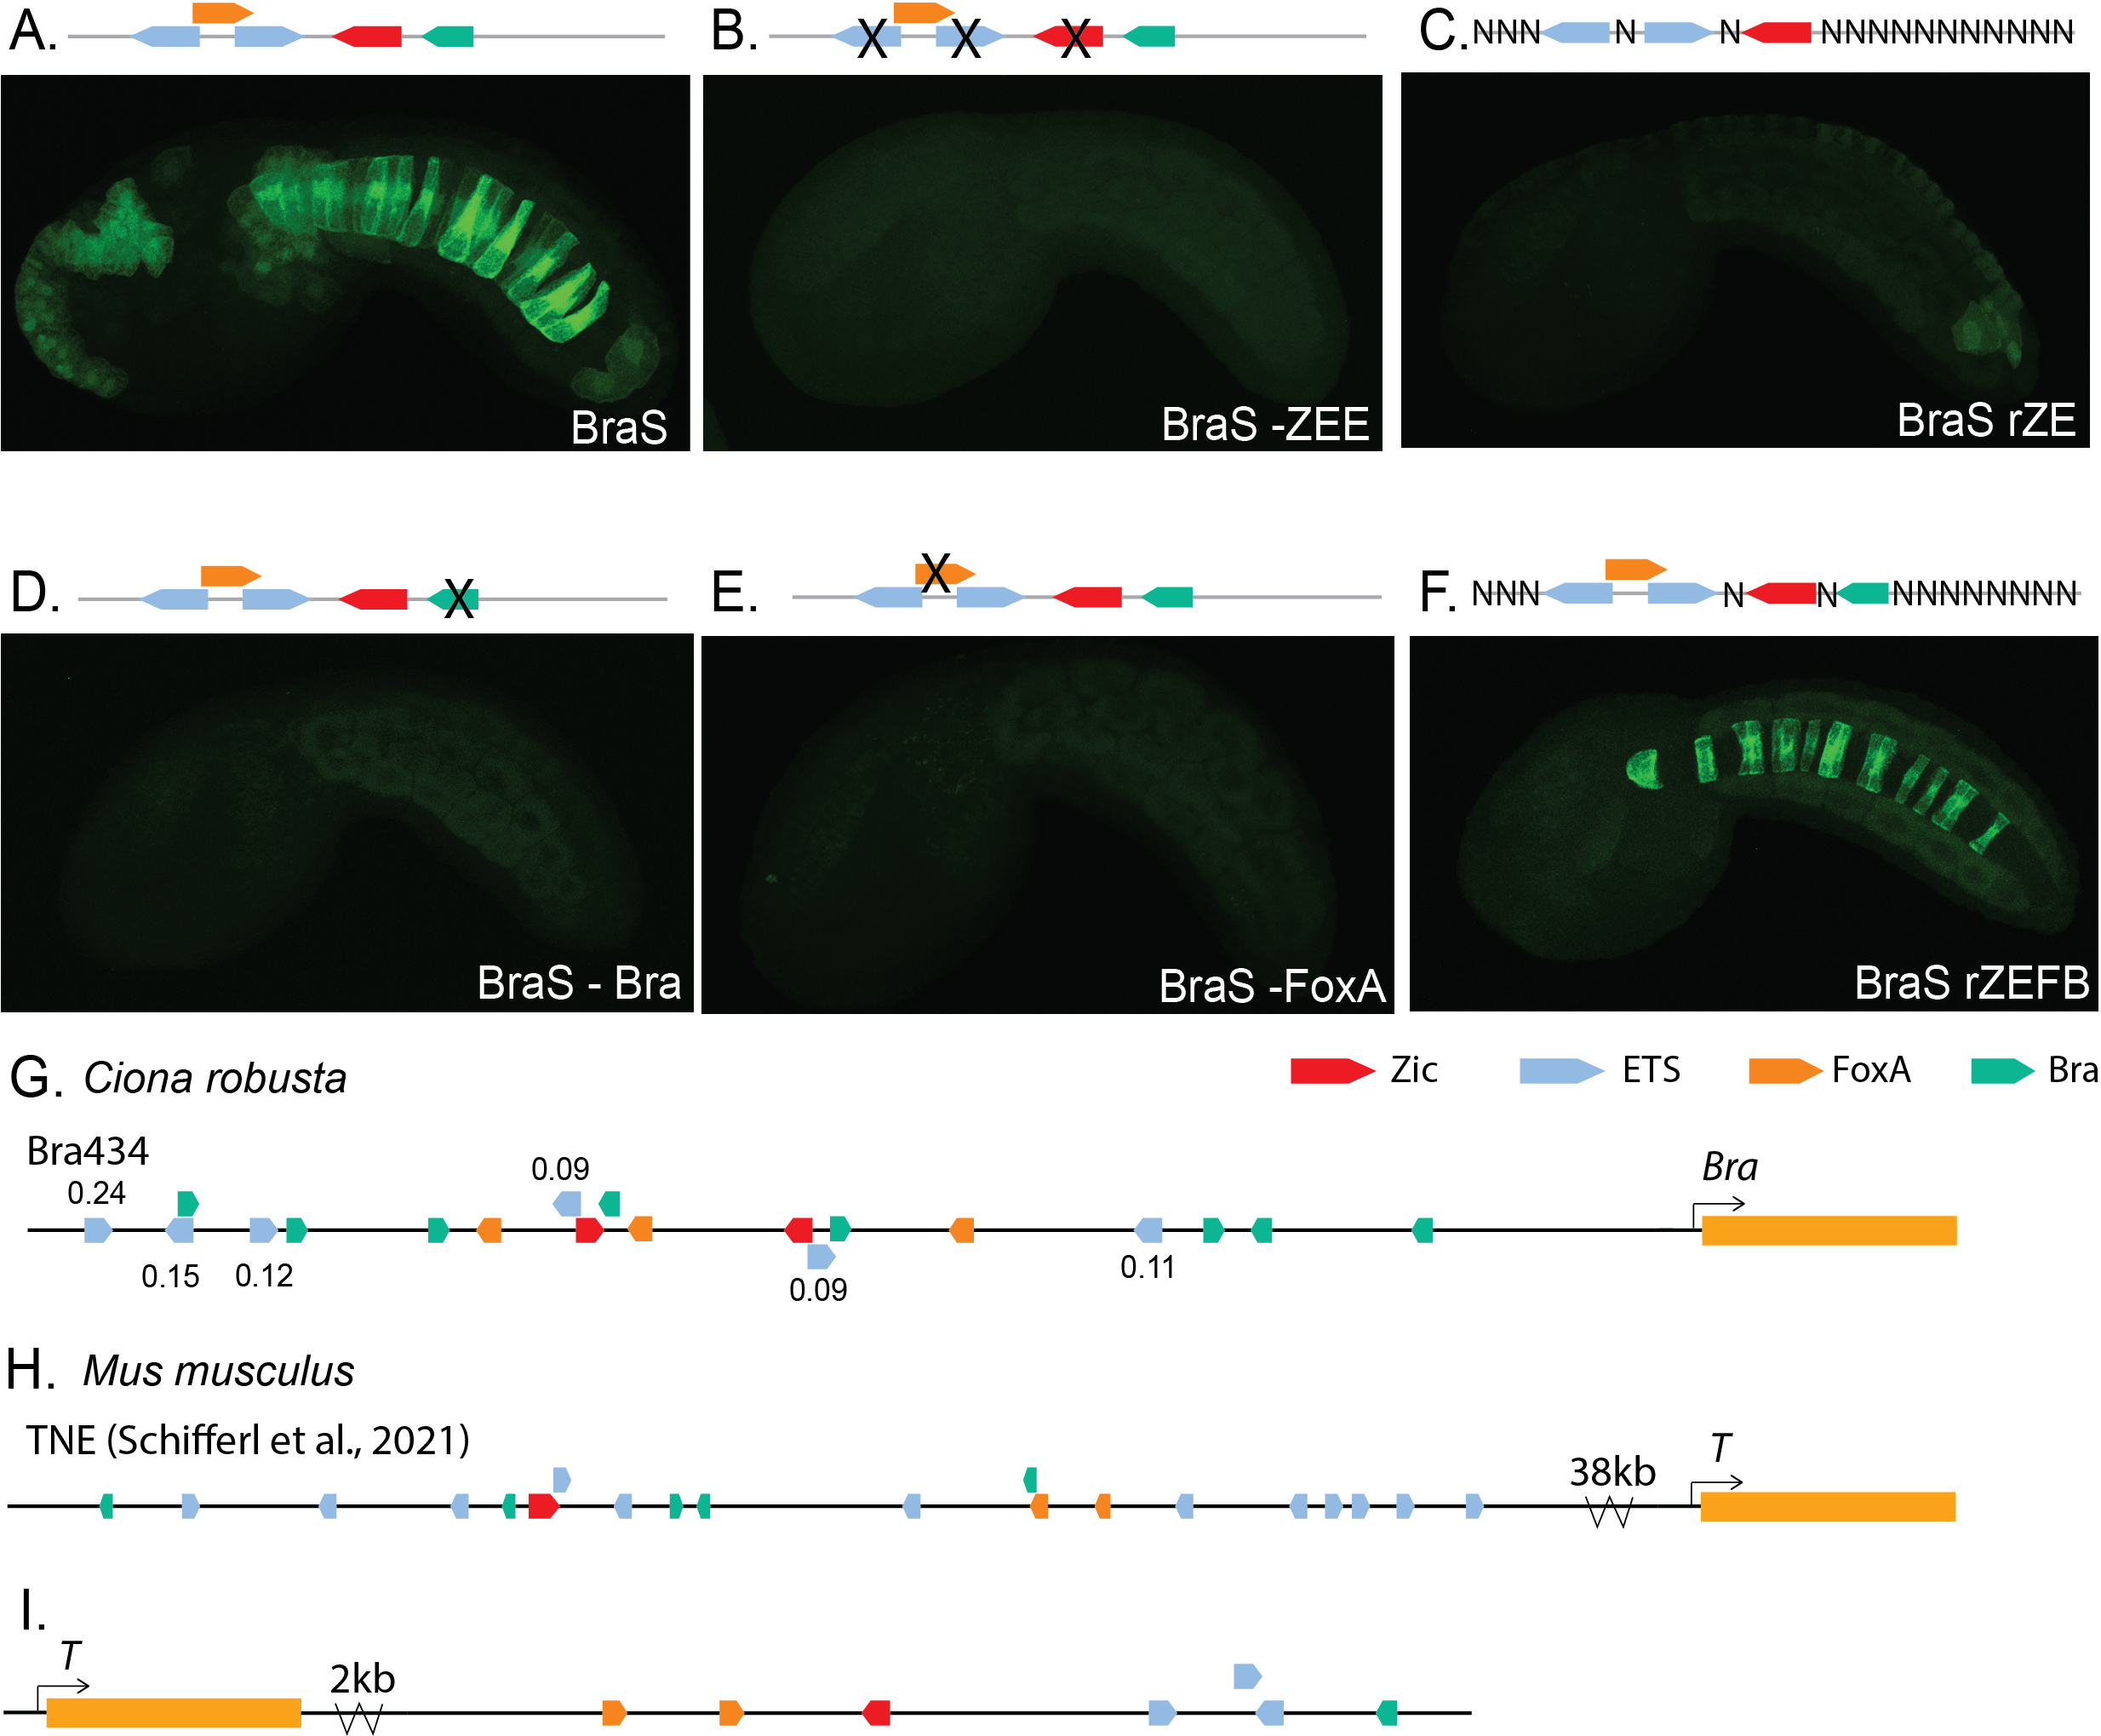
\includegraphics[scale=.74]{2_figures/Fig5_BraS-Dissection.png}
    \caption[Zic, ETS, FoxA, and Bra may be a common regulatory logic for \textit{Brachyury} enhancers]{\textbf{Zic, ETS, FoxA, and Bra may be a common regulatory logic for \textit{Brachyury} enhancers.} \textbf{A.} Embryo electroporated with the Bra Shadow (BraS) enhancer; GFP expression can be seen in the notochord. \textbf{B.} Embryo electroporated with BraS -ZEE, where the Zic and two ETS sites were mutated to be non-functional; no GFP expression was detected. \textbf{C.} Embryo electroporated with BraS rZE, where the Zic and two ETS sites were fixed, and all other nucleotides were randomized; GFP expression was greatly diminished. \textbf{D.} Embryo electroporated with BraS -Bra, where the sequence of Bra was mutated to be non-functional; GFP expression was greatly diminished. \textbf{E.} Embryo electroporated with BraS -FoxA, where the sequence of FoxA was mutated to be non-functional; GFP expression was greatly diminished. \textbf{F.} Embryo electroporated with BraS rZEFB, where the Zic, two ETS, FoxA, and Bra sites were fixed, and all other nucleotides were randomized; GFP expression can be seen in the notochord \textbf{G-I.} Schematics of Zic (red), ETS (blue), FoxA (orange), and Bra (green) clusters near Bra in the genomes of \textit{Ciona} and mouse. }
    \label{fig:5 brachyury shadow dissection}
\end{figure}

\subsection{Zic, ETS, Bra and FoxA may be a common regulatory logic for \textit{Ciona} \textit{Brachyury} enhancers}

The first and most well-studied Bra enhancer is the Bra434 enhancer \cite{corbo1997,fujiwara1998}, which drives strong expression in the notochord (Figure ~\ref{fig:supplement bra434 annotated}A).  Bra434 enhancer contains Zic, ETS, FoxA, and Bra sites; ablating these sites within this enhancer lead to reduced expression, suggesting that these sites contribute to enhancer activity \cite{reeves2021,shimai2022}. There are different reports regarding the number and location of Zic, ETS, FoxA, and Bra sites within the Bra434 enhancer depending on the method used to define sites \cite{corbo1997,shimai2022}. Here we annotate the Bra434 enhancer using crystal structure data, enhancer mutagenesis data, EMSA and PBM data \cite{casey1998,conlon2001,digregorio1999,dunn2009,katikala2013,lamber2008,li2017,matsumoto2007a,muller1997,passamaneck2009a,takahashi1999,wei2010,yagi2004}. 

Our approach identifies two Zic sites, six low-affinity ETS sites, three FoxA sites, and eight Bra sites (Figure ~\ref{fig:5 brachyury shadow dissection}G and Figure ~\ref{fig:supplement bra434 annotated}B). Of these TFs, the least information is available regarding Zic; thus, it is possible that there are other more degenerate Zic sites that may be identified in future studies \cite{corbo1997,fujiwara1998,reeves2021,shimai2022}. Bra434 has stronger expression in the notochord than BraS and this may be due to the longer length of the Bra434 enhancer and the presence of more Zic, ETS, FoxA and Bra sites within Bra434 relative to BraS enhancer. Having seen that clusters of Zic, ETS, FoxA, and Bra are important in the BraS and Bra434 enhancers, we next wanted to see if this logic is found in Bra enhancers in vertebrates.

\subsection{Vertebrate notochord enhancers contain clusters of Zic, ETS, Fox and Bra, suggesting this is a common logic for regulation of \textit{Brachyury} expression in the notochord}

In mouse, the most well-defined notochord enhancer to date is within an intron of T2, 38kb upstream of T, which is the mouse ortholog of Bra (Figure ~\ref{fig:5 brachyury shadow dissection}H) \cite{schifferl2021}. This mouse T enhancer is required for \textit{Bra/T} expression, notochord cell specification and differentiation \cite{schifferl2021}. Homozygous deletion of this \textit{Bra/T} enhancer in mouse leads to reduction of \textit{Bra/T} expression, a reduction in the number of notochord cells, and halving of tail length. Bra/T and FoxA binding sites have previously been identified within this enhancer \cite{schifferl2021}. We find that this mouse \textit{Bra/T} enhancer also contains Zic and ETS binding sites. Within this enhancer there are 12 ETS sites; 11 of these have affinities ranging from 0.09-0.14, while one site has an affinity of 0.65, indicating that this enhancer contains low-affinity ETS sites. 

As we saw with the \textit{Ciona} BraS and Bra434 enhancer, typically there are multiple enhancers that all regulate the same or similar patterns of expression \cite{frankel2010,hong2008,perry2010}. This is thought to confer the transcriptional robustness required for successful development \cite{antosova2016,frankel2010,osterwalder2018,perry2010}. Following this logic, we continued to search the mouse \textit{Bra/T} region to see if we could find other putative notochord enhancers that may regulate \textit{Bra/T}. We identified a region located 2kb downstream of T that contains a cluster of Zic, low-affinity ETS (0.11-0.12), FoxA and Bra sites (Figure ~\ref{fig:5 brachyury shadow dissection}I). This putative enhancer occurs within an open chromatin region in mouse E8.25 notochord cells \cite{pijuan-sala2020}, suggesting this may be another mouse T enhancer. Similarly in zebrafish, a notochord enhancer located 2.1kb upstream of the Bra ortholog \textit{ntl} \cite{harvey2010} also contains a cluster of Zic, ETS, FoxA, and Bra sites (Table S6). The presence of these four TFs in Ciona, zebrafish, and mouse Bra enhancers suggests that the use of Zic, ETS, FoxA and Bra could be a common enhancer logic regulating expression of the key notochord-specification gene Bra in chordates.

%%%%%%%%%%%%%%%%%%%%%%%%%%%%%%%%%%%%%%%%%%%%%%%%%%%%%%%%%%%%%%%%%%%%%%%%%%%%%%%%
\section{Discussion}
%%%%%%%%%%%%%%%%%%%%%%%%%%%%%%%%%%%%%%%%%%%%%%%%%%%%%%%%%%%%%%%%%%%%%%%%%%%%%%%%

In this study we sought to understand the regulatory logic of notochord enhancers by taking advantage of high-throughput studies within the marine chordate \textit{Ciona}. Within the \textit{Ciona} genome, there are 1,092 genomic regions containing a Zic site within 30 bp of two ETS sites. We tested 90 of these ZEE genomic regions for expression in developing \textit{Ciona} embryos. Surprisingly, only nine of the regions drove notochord expression. Among these nine, we identified a \textit{laminin alpha} enhancer that was highly dependent on grammatical constraints for proper expression. We found a similar cluster of Zic and ETS sites within the intron of the mouse and human \textit{laminin alpha-1} gene; strikingly, these clusters and the \textit{Ciona} laminin enhancer have the same spacing between the Zic and ETS sites. Within the BraS enhancer, although Zic and ETS are necessary for enhancer activity, randomization of the BraS enhancer keeping only the Zic and ETS sites constant in a sea of 24.5 million variants reveals that these sites are not sufficient for notochord activity. FoxA and Bra sites are also necessary for notochord expression. Indeed, creating a library of 45 million BraS variants in which all five TFBSs are kept constant in position, and affinity while all other nucleotides are randomized leads to notochord expression in a similar proportion of embryos as the WT BraS, which indicates these sites are sufficient for notochord expression . We find that the combination of Zic, ETS, FoxA, Bra occurs within other Bra enhancers in \textit{Ciona} and vertebrates suggesting this combination of TFs may be a common logic regulating Bra expression. Our study identifies new developmental enhancers, demonstrates the importance of enhancer grammar within developmental enhancers and provides a deeper understanding of the regulatory logic governing Bra. Our findings of the same clusters of sites within vertebrates hint at the conserved role of grammar and logic across chordates. 

\subsection{Very few genomic regions containing Zic and two ETS sites are functional enhancers}

Our analysis of 90 genomic elements all containing at least one Zic site in combination with two ETS sites strikingly demonstrated that clusters of sites are not sufficient to drive expression. Only 39 of the 90 (43\%) elements tested drove any expression, and even more surprisingly, only 15 of these drove expression in lineages that co-express Zic and ETS, namely the a6.5 (anterior sensory vesicle and palps) and/or notochord. These findings indicate that searching for clusters of TFs is only minimally effective in identification of enhancers and suggests that the organization of sites is also important for rendering a cluster of binding sites a functional enhancer. Our findings are in agreement with the work from King et al., that found only 28\% of the genomic elements they tested for enhancer function in ES cells drove enhancer activity, despite the fact that these genomic elements contain TF motifs and bound these TFs in ChIP-seq assays \cite{king2020a}. Our study and King et al. suggest that having motifs, or even TF binding is not sufficient to drive expression and suggests that the grammar of these sites is critical for rendering a cluster of TFBSs a functional enhancer \cite{king2020a}. 

\subsection{Grammar is a key constraint of the Lama and BraS enhancers} 

Zic and ETS are necessary for activity of the Lama enhancer. Within the Lama enhancer, the orientation of binding sites relative to each other was critical for expression, providing evidence that enhancer grammar is a critical feature of functional enhancers regulated by Zic and ETS. Flipping the orientation of either the first or last ETS sites relative to the Zic site led to loss of enhancer activity in the \textit{Ciona} Lama enhancer. This mirrors the results of flipping the orientation of the ETS sites within the BraS enhancer \cite{farley2016}. \textit{Laminin alpha} is a key gene involved in notochord development in both \textit{Ciona} and vertebrates \cite{pollard2006,veeman2008}. Intriguingly, we find that both the human and mouse \textit{laminin alpha-1} have introns that harbor a similar cluster of Zic and ETS sites to those seen within \textit{Ciona}. There is a conservation of 12 bp spacing between the Zic and ETS site across all three chordate enhancers, similar to the spacing we have observed between Zic and ETS sites within the notochord enhancers Mnx and BraS \cite{farley2016}. We note that the vertebrate regions do not drive notochord expression in \textit{Ciona}. It possible that grammar is subtly tweaked between different species. Alternatively, the lack of activity could be due to promoter incompatibility across species, as in our assay we tested the mouse and human Lama enhancers with a \textit{Ciona} promoter. Reporter assays within mouse embryos could further investigate the functionality of the mouse and human Lama putative enhancers and the role of the 12 bp spacing within these elements.   

\subsection{Necessity of sites does not mean sufficiency--a deeper understanding of the BraS enhancer}

Our study of the BraS enhancer highlights the importance of testing sufficiency of sites to investigate if we fully understand the regulatory logic of an enhancer. We previously demonstrated that reversing the orientation of an ETS site led to loss of notochord expression in the BraS enhancer. Here, in this study, we show via point mutations that both Zic and ETS sites are required for enhancer activity. However, randomization of the BraS enhancer to create 24.5 million variants in which only the Zic and ETS sites are constant demonstrates that these sites are not sufficient for enhancer activity, as the randomized BraS enhancer (BraS rZE) only drives notochord expression in less than half the number of embryos as the BraS enhancer. Having discovered that Zic and ETS alone were not sufficient, we find that both FoxA and Bra sites also contribute to the enhancer activity. In a library of 45 million variants in which the Zic, ETS, Bra and FoxA sites are kept constant in sequence, affinity and position within a randomized backbone (BraS rZEFB), we see no significant difference in the number of embryos with notochord expression. This indicates that these five sites are necessary and sufficient for enhancer activity. However, the neural expression seen with the BraS enhancer appears to depend on some features within the randomized backbone, as the ZEFB library drives significantly less neural expression. We also note that the BraS rZEFB drives slightly weaker levels of notochord expression. These findings illustrate that enhancers are densely encoded with many features which contribute to expression. This is in line with recent work suggesting that enhancers contain far more regulatory information that previously appreciated \cite{fuqua2020}. It is possible that degenerate Zic, ETS, FoxA, or Bra sites could be present or novel TFBS are also contributing to this logic. Further analysis conducting MPRAs with these two libraries (BraS rZE and BraS rZEFB) will determine what other features are contributing to  notochord and neural expression. Sufficiency experiments are rarely done, and we are unaware of another study that has tested sufficiency across the entirety of an enhancer in developing embryos. However, our experiments demonstrate the importance of testing sufficiency to determine all the features contributing to enhancer function and illustrate the dense encoding of regulatory information within enhancers. 

\subsection{Partial grammatical rules can provide signatures that identify enhancers, but improved understanding could lead to more accurate predictions}

We were able to find the BraS enhancer using grammatical constraints on organization and spacing between Zic and ETS site and affinity of ETS sites \cite{farley2016}. Interestingly, we did not have all the features required for enhancer activity. As such, this suggests that partial knowledge of grammatical constraints, or partial signatures of grammar could be used to identify functional enhancers. Our previous strategy searched for these grammatical constraints in proximity of known notochord genes, which may be why we were successful in identification of the Mnx and BraS enhancer with only partial grammar rules. Understanding the dependency between all features within an enhancer will likely enable greater success in identification of functional regulatory elements, as current genomic screens have shown limited success of identifying functional enhancers through epigenetic markers and transcription factor binding sites alone \cite{king2020a}. Until then, our current knowledge of grammatical constraints may still be useful for pointing us towards putative enhancers. 

\subsection{Zic, ETS, FoxA, and Bra may be a common logic upstream of \textit{Brachyury} in chordates}

The Bra434 enhancer also contains the same combination of sites as the BraS enhancer; therefore, it is possible that this is a common logic for regulating Bra. Interestingly, we find these sites within mouse and zebrafish Bra enhancers \cite{harvey2010,schifferl2021}. While there are differences in expression dynamics of these factors in vertebrates and ascidians, it is striking to see this combination of sites in validated notochord enhancers across these species. Indeed, our study in both the laminin enhancers and Bra enhancers provides hints of a conserved regulatory logic across chordates, although future tests of these putative enhancers within mouse are required to see if these are truly conserved enhancers with similar grammar signatures. Our study focuses on conservation of grammatical signatures rather than sequence conservation. A recent study searching for conserved enhancers in syntenic regions suggests that there may be much more conservation of enhancer function than expected based on sequence conservation \cite{wong2020}. Our approach searching for grammatical signatures rather than sequence conservation may allow for identification of such functionally conserved enhancers.

\subsection{Approaches to understanding dependency grammar of notochord expression}

Searching for grammatical rules governing enhancers requires comparison of functional enhancers with the same features. Although we thought we had the same features in all 90 regions, we actually had at least three distinct types of enhancers within our screen. This illustrates a common problem in mining genomic data for patterns, as the assumption that we are comparing like with like is often an incorrect one. Other screens mining genomic elements have hit similar roadblocks, with only a few functional genomic examples being uncovered and thus limiting the ability to find grammatical rules \cite{king2020a}.  To uncover the grammatical constraints on enhancers, we need to not only understand the number and types of sites within an enhancer, but also the dependency between these sites, such as affinity, spacing, and orientation \cite{jindal2021}. 

Massively or gigantic parallel reporter assays with increased size and complexity and that combine both synthetic enhancers and genomic elements will likely be required to pinpoint the rules governing enhancer activity within genomes. However, integrating synthetic screens with genomic screens is a major challenge as synthetic screens often have limited application within the context of the genome \cite{king2020a}. Another approach is to study entirely random sequences for enhancer activity, which has been done in the context of promoters in bacteria and yeast \cite{yona2018,deboer2020a}. Indeed, the conclusions of these studies mirror our own findings that grammar and low-affinity sites are critical components of functional regulatory elements. However, as 83\% of the random sequences within yeast drove expression, it is unclear how well random sequences mirror the regulatory landscape within the genome that has been shaped by evolutionary constraints over millions of years. Nonetheless, testing random sequences within the context of developing embryos could provide another source of data to understand how enhancers encode tissue-specific expression \cite{galupa2022}. In the future, integration of genomic regions, synthetic designed, and random sequences will contribute to our understanding of enhancer grammar. Despite the complexity of studying enhancers in developing embryos, our study demonstrates that enhancer grammar is critical for encoding notochord activity and our observation of the same logics and grammar signatures in both \textit{Ciona} and vertebrates hints at conservation of these grammatical constraints across chordates. 

\subsection{Limitations of the study}

In this study, we screened 90 ZEE elements for functionality; however, only 10\% were active in the notochord. We anticipate that discovering more notochord enhancers regulated by Zic, ETS, or regulated by Zic, ETS, FoxA, and Bra could better inform our understanding of notochord grammar. Towards this end, testing all 1,092 ZEE elements we identified within the \textit{Ciona} genome could strengthen this study. However, this would likely only yield 100 notochord enhancers, which would still not be enough to define grammatical rules. As discussed above, combining assays of genomic regions with synthetic and random enhancer screens could help gain enough data to determine the grammar of notochord enhancers. 

Another limitation relates to our identification of conserved enhancer logic and grammar across chordates. While we identified similar signatures with the Lama enhancers in Ciona, mouse and humans, we did not test the mouse Lama enhancer for activity in mouse, nor did we functionally interrogate the importance of the 12 bp spacing within this enhancer in the context of \textit{Ciona} or mouse. Conducting these studies would deepen our understanding of the conservation of grammar across chordates. We also identified a common logic of Zic, ETS, FoxA and Bra within Bra enhancers. While we know that deletion of the mouse Bra TNE enhancer does lead to loss of notochord in mouse, it would strengthen the study to manipulate the Zic, ETS, FoxA, Bra sites within the context of the mouse and zebrafish Bra/T enhancers to determine if the conservation of this logic is important for regulation of Bra.

%%%%%%%%%%%%%%%%%%%%%%%%%%%%%%%%%%%%%%%%%%%%%%%%%%%%%%%%%%%%%%%%%%%%%%%%%%%%%%%%
\section{STAR*Methods}
%%%%%%%%%%%%%%%%%%%%%%%%%%%%%%%%%%%%%%%%%%%%%%%%%%%%%%%%%%%%%%%%%%%%%%%%%%%%%%%%

%%% %%% %%% %%% %%% %%% %%% %%% %%% %%% %%% %%% %%% %%% %%% %%% %%% %%% %%% %%%
\subsection{Key resources table}

\begin{landscape} % this table is long, so it'll be multi-page landscape
    \begin{longtable}{p{.49\textwidth} p{.35\textwidth} p{.5\textwidth}}
        % Define the table title in the table of contents
        \caption{Key resources table} \\ \hline 

        % Define the table columns for the first and all subsequent pages
        \multicolumn{1}{l}{\textbf{REAGENT or RESOURCE}} & \multicolumn{1}{l}{\textbf{SOURCE}} & \multicolumn{1}{l}{\textbf{IDENTIFIER}} \\ \hline \endfirsthead

        \multicolumn{3}{l}%
        {{\textbf{\tablename\ \thetable{}}, \textit{continued from previous page}}} \\
        \hline 
        \multicolumn{1}{l}{\textbf{REAGENT or RESOURCE}} & \multicolumn{1}{l}{\textbf{SOURCE}} & \multicolumn{1}{l}{\textbf{IDENTIFIER}} \\ \hline\hline \endhead

        % Define the table footer for the first and all subsequent pages
        \hline \multicolumn{3}{r}{\textit{Continued on next page}} \\ \hline \endfoot
        \hline \endlastfoot
        
        % Start table content

        %%%%% %%%%% %%%%% %%%%% %%%%% %%%%% %%%%% %%%%% %%%%% %%%%% %%%%% %%%%%
        \textit{Deposited Data} \\ \hline
        snATACseq mouse E8.25 & Pijuan-Sala et al., 2020\cite{pijuan-sala2020} & GEO: \href{https://www.ncbi.nlm.nih.gov/geo/query/acc.cgi?acc=GSE133244}{GSE133244} \\ 
        FACS-sorted notochord RNA-Seq & Reeves et al., 2017\cite{reeves2017} & N/A \\
        Human reference genome NCBI build 38 & Genome Reference Consortium & \href{https://www.ncbi.nlm.nih.gov/grc/human}{NCBI, Human GRCh38 Reference} \\
        Mouse reference genome NCBI build 39 & Genome Reference Consortium & \href{https://www.ncbi.nlm.nih.gov/grc/mouse}{NCBI, Mouse GRCm39 Reference} \\
        \textit{Ciona} robusta genome & Satoh et al., 2005\cite{satou2005} & \href{http://ghost.zool.kyoto-u.ac.jp/cgi-bin/gb2/gbrowse/kh/}{Ghost Database} \\
        mouse ETS-1 universal PBM data & Wei et al., 2010\cite{wei2010} & \href{https://thebrain.bwh.harvard.edu/uniprobe/index.php}{UniProbe Database} \\
        ZEE library screen & This paper & N/A \\
        
        %%%%% %%%%% %%%%% %%%%% %%%%% %%%%% %%%%% %%%%% %%%%% %%%%% %%%%% %%%%%
        \hline \textit{Experimental Models: Organisms/Strains} \\ \hline
        \textit{Ciona} intestinalis type A (\textit{Ciona} robusta) & M-Rep & N/A \\

        %%%%% %%%%% %%%%% %%%%% %%%%% %%%%% %%%%% %%%%% %%%%% %%%%% %%%%% %%%%%
        \hline \textit{Oligonucleotides} \\ \hline
        Oligonucleotides for library screen, see Table S1 & This paper & N/A \\
        Oligonucleotides for mutagenesis, see Table S4 & This paper & N/A \\

        %%%%% %%%%% %%%%% %%%%% %%%%% %%%%% %%%%% %%%%% %%%%% %%%%% %%%%% %%%%%
        \hline \textit{Recombinant DNA} \\ \hline
        Plasmid: BraS bpFog>GFP & Farley Lab & N/A \\ 
        Plasmid: BraS -ZEE bpFog>GFP & This paper & N/A \\
        Plasmid: BraS rZE bpFog>GFP & This paper & N/A \\
        Plasmid: BraS -FoxA bpFog>GFP & This paper & N/A \\
        Plasmid: BraS -Bra bpFog>GFP & This paper & N/A \\ 
        Plasmid: BraS rZEFB bpFog>GFP & This paper & N/A \\
        Plasmid: Lama1 bpFog>GFP & This paper & N/A \\
        Plasmid: Lama1 bpFog>GFP & This paper & N/A \\
        Plasmid: Lama1 -E3 bpFog>GFP & This paper & N/A \\
        Plasmid: Lama1 -Z bpFog>GFP & This paper & N/A \\
        Plasmid: Lama1 RE3 bpFog>GFP & This paper & N/A \\

        %%%%% %%%%% %%%%% %%%%% %%%%% %%%%% %%%%% %%%%% %%%%% %%%%% %%%%% %%%%%
        \hline \textit{Software and Algorithms} \\ \hline
        Python (version 3.8.6)  & Python Software Foundation & \href{https://www.python.org}{https://www.python.org} \\
        Conda (version 4.9.2) & Anaconda, Inc. & \href{https://docs.conda.io/}{https://docs.conda.io} \\
        Bioconda  & Grüning et al., 2018 & \href{https://bioconda.github.io}{https://bioconda.github.io} \\
        Biopython (version 1.78) & Cock et al., 2009 & \href{https://biopython.org}{https://biopython.org} \\
        FastQC (version 0.11.9)	& Babraham Institute & \href{https://www.bioinformatics.babraham.ac.uk/}{https://www.bioinformatics.babraham.ac.uk} \\
        MultiQC (version 1.8) & Ewels et al., 2016 & \href{https://multiqc.info}{https://multiqc.info} \\
        FLASH (version 1.2.11) & Magoč et al., 2011 & \href{http://www.cbcb.umd.edu/software/flash}{http://www.cbcb.umd.edu/software/flash} \\
        \verb|pandas| (version 1.2.1) & NumFOCUS & \href{https://pandas.pydata.org}{https://pandas.pydata.org} \\
        \verb|numpy| (version 1.20.3) & Harris et al., 2020 & \href{https://numpy.org}{https://numpy.org} \\
        \verb|matplotlib| (version 3.2.2) & Hunter, 2007 & \href{https://matplotlib.org/}{https://matplotlib.org} \\
        \verb|scikit-learn| (version 0.24.1) & Pedregosa et al., 2011 & \href{https://scikit-learn.org/}{https://scikit-learn.org} \\
        \verb|seaborn| (version 0.11.1) & Waskom et al., 2021 & \href{https://seaborn.pydata.org/}{https://seaborn.pydata.org} \\
        \verb|Diverse-Logics-Notochord-Study| & Code used in this paper & \href{https://github.com/mragsac/Diverse-Logics-Notochord-Study}{Diverse-Logics-Notochord-Study GitHub} \\
    \end{longtable}
\end{landscape}

%%% %%% %%% %%% %%% %%% %%% %%% %%% %%% %%% %%% %%% %%% %%% %%% %%% %%% %%% %%%
\subsection{Resource availability}

%%% %%% %%% %%% %%% %%% %%% %%% %%% %%% %%% %%% %%% %%% %%% %%% %%% %%% %%% %%%
\subsubsection{Lead contact} 
Further information and requests for resources and reagents should be directed to and will be fulfilled by the lead contact, Emma K. Farley (\href{mailto:efarley@ucsd.edu}{efarley@ucsd.edu}). 

%%% %%% %%% %%% %%% %%% %%% %%% %%% %%% %%% %%% %%% %%% %%% %%% %%% %%% %%% %%%
\subsubsection{Materials availability} 
Plasmids generated in this study are available upon request. 

%%% %%% %%% %%% %%% %%% %%% %%% %%% %%% %%% %%% %%% %%% %%% %%% %%% %%% %%% %%%
\subsection{Experimental model and subject details}
\subsubsection{Tunicates}
Adult \textit{\textit{Ciona} intestinalis type A}, also known as \textit{\textit{Ciona} robusta}, were obtained from M-Rep and were maintained under constant illumination in seawater (obtained from Reliant Aquariums) at $18^\circ$C. \textit{Ciona} are hermaphroditic, therefore there is only one possible sex for individuals. Age or developmental stage of the embryos studied are indicated in the main text. 

%%% %%% %%% %%% %%% %%% %%% %%% %%% %%% %%% %%% %%% %%% %%% %%% %%% %%% %%% %%%
\subsection{Method details}
\subsubsection{Library Construction}
The genomic regions were ordered from Agilent Technologies with adapters containing BseRI sites. This was cloned into the custom-designed SEL-Seq (Synthetic Enhancer Library-Sequencing) vector using type II restriction enzyme BseRI. After cloning, the library was transformed into bacteria (MegaX DHB10 electrocompetent cells), and the culture was grown up until an OD of 1 was reached. DNA was extracted using the Macherey-Nagel Nucleobond Xtra Midi kit. A 30 bp barcode with adapters containing Esp3I sites was cloned into this library using type II restriction enzyme Esp3I. The library was transformed into bacteria (MegaX DHB10 electrocompetent cells) and grown up until an OD of 2 was reached. The DNA library was extracted from the bacteria using the Macherey-Nagel Nucleobond Xtra Midi kit. 

\subsubsection{Electroporation}
Dechorionation, \textit{in vitro} fertilization, and electroporation were performed as described previously in Farley et al., 2016.

\subsubsection{GFP reporter assays}
70 $\mu$g DNA was resuspended in 100 $\mu$L water and added to 400 $\mu$L of 0.96 M D-mannitol. Typically for each electroporation, eggs and sperm were collected from 10 adults. Embryos were fixed at the appropriate developmental stage for 15 minutes in 3.7\% formaldehyde. The tissue was then cleared in a series of washes of 0.3\% Triton-X in PBS and then of 0.01\% Triton-X in PBS. Samples were mounted in Prolong Gold. GFP images were obtained with an Olympus FV3000, using the 40X objective. All constructs were electroporated in three biological replicates.

\subsubsection{ZEE MPRA screen}
50 $\mu$g of the ZEE library was electroporated into ~5,000 fertilized eggs. Embryos developed until 5 hours and 30 minutes at $22^\circ$C. Embryos put into TriZol, and RNA was extracted following the manufacturer's instructions (Life Technologies). The RNA was DNase treated using Turbo DNaseI from Ambion following standard instructions. Poly-A selection was used to obtain only mRNA using poly-A biotinylated beads as per instructions (Dyna-beads, Life technologies). The mRNA was used in an RT reaction that was specifically selected for the barcoded mRNA (Transcriptor High Fidelity, Roche). The RT product was PCR amplified and size selected using Agencourt AMPure beads (Beckman Coulter), then checked for quality and size on the 2100 Bioanalyzer (Agilent) and sent for sequencing on the NovaSeq S4 PE100 mode (Illumina). Three biological replicates were sent for sequencing. 

The DNA was extracted by mixing the phenol-chloroform and interphase of TriZol extraction with 500 $\mu$L of Back Extraction Buffer (4 M guanidine thiocyanate, 50 mM sodium citrate, and 1 M Tris-base). DNA was treated with RnaseA (Thermo Fisher). DNA was cleaned up with phenol:chloroform:isoamyl alcohol (25:24:1) (Life Technologies). The DNA was PCR amplified and size selected using Agencourt AMPure beads (Beckman Coulter), then checked for quality and size on the 2100 Bioanalyzer (Agilent) and sent for sequencing on the NovaSeq S4 PE100 mode (Illumina). Three biological replicates were sent for sequencing.

\subsubsection{Counting Embryos}
For each experiment, once embryos had been mounted on slides, slide labels were covered with thick tape and randomly numbered by a laboratory member not involved in this project. Expression of GFP within embryos on each slides was counted blind. In each experiment, all comparative constructs were present, along with a slide with BraS as a reference. The X-Cite was turned on for 1hr before analysis to ensure the illumination intensity was constant. To determine levels of expression, high expression was set as visible with less than 25\% power on X-Cite illuminator. Fifty embryos were counted for each biological replicate.

\subsubsection{Acquisition of Images}
For enhancers being compared, images were taken from electroporations performed on the same day using identical settings. For representative images, embryos were chosen that represented the average from counting data. All images are subsequently cropped to an appropriate size. In each figure, the same exposure time for each image is shown to allow direct comparison.

\subsubsection{Identification of Putative Notochord Enhancers}
We developed a script that allows for the input of any organism’s genome in the fasta file format. The script first looks for an exact match of one of seven canonical Zic family binding sites and their reverse complements. We used the following sites in our search: \verb|CAGCTGTG| (Zic1/2/3), \verb|CCGCAGT| (Zic7/3/1), \verb|CCGCAGTC| (Zic6), \verb|CCCGCTGTG| (Zic1), \verb|CCAGCTGTG| (Zic3), \verb|CCGCTGTG| (Zic2/ZicC), and \verb|CCCGCAGTC| (Zic5) as these have been identified as functional in previous studies (Matsumoto et al., 2007a; Yagi et al., 2004). Next, we drew a window of 30 bp from either end of the canonical Zic family binding site and determine if there are at least two Ets binding site cores (i.e., either \verb|GGAA| or \verb|GGAT| and their respective reverse complement sequences) present within the window. The location of all regions containing at least a single Zic family binding site and two Ets binding sites are saved as part of the genome search.

\subsubsection{Scoring Relative Affinities of Binding Sites}
We calculated the relative ETS binding affinity using the median signal intensity of the universal protein binding microarray (PBM) data for mouse Ets-1 proteins from the UniProbe database (\href{http://thebrain.bwh.harvard.edu/uniprobe/index.php}{http://thebrain.bwh.harvard.edu/uniprobe/index.php}) (Hume et al., 2015). Previous studies have shown that the specificity of ETS family members is highly conserved even from flies to humans (Nitta et al., 2015; Wei et al., 2010), and thus ETS-1 is a good proxy for binding affinity in \textit{Ciona} ETS-1 which has a conserved DNA binding domain (Farley et al., 2015). The relative affinity score represents the fractional binding of median signal intensities of the native 8-mer motifs compared to the optimal 8-mer motifs for optimal Ets, which we defined as the \verb|CCGGAAGT| motif and its corresponding reverse complement.  

\subsubsection{Enhancer to Barcode Assignment \& Dictionary Analysis}
We constructed a dictionary of unique barcode tag-enhancer pairs by not allowing for any mismatches in the ~68 bp enhancers in our library and by not allowing barcode tag-enhancer pairs to have a read count of fewer than 150 reads. Additionally, we required all barcode tags to be 29 bp or 30 bp in length. If more than one barcode tag was associated with a single enhancer, we included all associated barcode tags that met the aforementioned barcode length and read count requirements. Within our dictionary, we did not find barcode tags that were matched to multiple enhancers. In total, the dictionary contains 90 enhancers that were uniquely mapped to one or more barcode tags, and a total of 640 barcode tag-enhancer pairs.

\subsubsection{SEL-Seq Data Analysis}
For the whole embryo library, we sequenced barcode tags from the DNA and RNA libraries on the Illumina HiSeq 4000. Reads that perfectly matched barcode tags in our barcode tag-enhancer dictionary were included in the subsequent analysis.
We extracted all of the read sequences from the sequencing libraries and collapse them based on unique sequences, tabulating the number of times a unique sequence appears in the library. Next, we perform preliminary filtering on the unique sequences, filtering out sequences that (i) have N’s present, (ii) are missing the GFP sequence after our expected location of the barcode tag, (iii) contain a barcode that is not an exact match to our enhancer-barcode tag dictionary, (iv) did not meet the minimum read cutoff of 25 reads. For the preliminary filtering step, all DNA and RNA libraries were processed separately. 

We normalize our data into RPM.  We filter our data to only include the set of barcode tags and enhancers that appear in DNA across all replicates and consolidate the expression for each enhancer by taking the average RPM value across barcode tags. For determining if an enhancer was active, we calculated an “enhancer activity score.” This score is calculated by averaging the $log_2({\frac{RNA}{DNA}})$ value across a given enhancer’s biological replicates. 

%%% %%% %%% %%% %%% %%% %%% %%% %%% %%% %%% %%% %%% %%% %%% %%% %%% %%% %%% %%%
\subsection{Quantification and statistical analysis}

To assess statistical differences between enhancer expression, Fischer’s exact test was used with the \verb|fisher.test| function in the R programming language. To assess statistical differences between enhancer expression levels, chi-squared test was used with the \verb|CHISQ.TEST| function in Microsoft Excel.

%%%%%%%%%%%%%%%%%%%%%%%%%%%%%%%%%%%%%%%%%%%%%%%%%%%%%%%%%%%%%%%%%%%%%%%%%%%%%%%%
\section{Data and code availability}
%%%%%%%%%%%%%%%%%%%%%%%%%%%%%%%%%%%%%%%%%%%%%%%%%%%%%%%%%%%%%%%%%%%%%%%%%%%%%%%%

Microscopy and scoring data reported in this paper will be shared by the lead contact upon request.

All ZEE screen sequencing data will be deposited to GEO and will be made publicly available as of the date of publication. The data will also be on SRA listed under the submission identifier \href{https://www.ncbi.nlm.nih.gov/sra/PRJNA861319}{PRJNA861319} and will be made available as of the date of publication. DOIs will be listed in the key resources table upon publication. 

All original code has been deposited to GitHub (\href{https://github.com/mragsac/Diverse-Logics-Notochord-Study}{https://github.com/mragsac/Diverse-Logics-Notochord-Study}) and is publicly available. DOIs will be listed in the key resources table upon publication. 

Any additional information required to reanalyze the data reported in this paper is available from the lead contact upon request. 

%%%%%%%%%%%%%%%%%%%%%%%%%%%%%%%%%%%%%%%%%%%%%%%%%%%%%%%%%%%%%%%%%%%%%%%%%%%%%%%%
\section{Acknowledgments}
%%%%%%%%%%%%%%%%%%%%%%%%%%%%%%%%%%%%%%%%%%%%%%%%%%%%%%%%%%%%%%%%%%%%%%%%%%%%%%%%

We thank the Farley Lab and Dennis Schifferl for helpful discussions. We thank Janet H.T. Song for her critical reading of the manuscript. We thank the UCSD IGM Genomics Center for their assistance with sequencing. B.P.S. was supported by NIH T32 GM133351. M.F.R. is supported by T32 GM008666. K.T. is supported by NSF 2109907 and 3DP2HG010013-01S1. G.A.J. was supported by a Hartwell Fellowship and NIH T32HL007444. E.K.F., B.P.S., M.F.R., K.T., G.A.J., J.L.G., S.H.L. were supported by NIH DP2HG010013.

% Include the acknowledgement that this is a reformatted reprint
Chapter 1,  in full,  is  a  reformatted  reprint  of  the  material as it appears in “Diverse logics encode notochord enhancers.”  Benjamin P. Song, Michelle F. Ragsac, Krissie Tellez, Granton A. Jindal, Jessica L. Grudzien, Sophia H. Le, Emma K. Farley. \textit{In Submission}, 2022.  The dissertation author was the primary investigator and co-first author of this paper.

%%% %%% %%% %%% %%% %%% %%% %%% %%% %%% %%% %%% %%% %%% %%% %%% %%% %%% %%% %%%
\subsection{Author contributions}
E.K.F., B.P.S., M.F.R, K.T., G.A.J. designed experiments. B.P.S., K.T., J.L.G., S.H.L. conducted experiments. M.F.R. conducted bioinformatic analyses. E.K.F. and B.P.S wrote the manuscript. All authors were involved in editing the manuscript.

%%% %%% %%% %%% %%% %%% %%% %%% %%% %%% %%% %%% %%% %%% %%% %%% %%% %%% %%% %%%
\subsection{Declaration of interests}
The authors declare no competing interests.
